\chapterimage{Pictures/chap08/dragons-fourier-600x1200.png}
\chapter{反射模型}\label{chap:反射模型}
\setcounter{sidenote}{1}
本章定义一组类来描述光在表面上散射的方式。回想\refsub{BRDF}中
我们介绍了双向反射分布函数(BRDF)抽象来描述表面的光反射,
双向透射分布函数(BTDF)来描述表面的透射,以及
双向散射分布函数(BSDF)来统合这两种效应。
本章中,我们将从为这些表面反射和透射函数定义通用接口开始。

许多来自表面的散射通常最好描述为多个BRDF和BTDF随空间变化的混合体;
在第\refchap{材质},我们将介绍结合了多个BRDF和BTDF的BSDF对象
以表示来自表面的整体散射。本章回避了反射和折射性质随表面变化的问题;
第\refchap{纹理}的纹理类将解决该问题。
BRDF和BTDF只显式建模了在表面上同一点入射和出射的光的散射。
对于展现出有意义的次表面光传输的曲面,我们将引入类\refvar{BSSRDF}{},
在第\refchap{体积散射}介绍一些相关理论后,它将在\refsec{BSSRDF}对次表面散射建模。

表面反射模型有以下几个来源:
\begin{itemize}
      \item \emph{测量的数据}:许多真实世界表面的反射分布性质已在实验室中测定。
            这样的数据可直接以表格形式使用或用来为一组基函数计算系数。
      \item \emph{现象模型}\sidenote{译者注:原文phenomenological models。}:
            试图描述真实世界表面定性性质的方程在仿真时可能很有效。
            这类BSDF可能很容易使用,因为它们常常有直观的参数来修改其表现(例如“粗糙度”)。
      \item \emph{模拟}:有时关于表面组成的底层信息是已知的。
            例如,我们可能知道涂料是悬浮在介质中的平均大小彩色颗粒组成的,
            或者某种布料是两种织线组成的,且知道每种的反射性质。
            在这些情况下,可以模拟来自微观几何体的光散射来生成反射数据。
            该模拟可在渲染时进行,或作为预处理完成后去适配一组基函数供渲染时使用。
      \item \emph{物理(波动)光学}:一些反射模型是用详细的光模型推导出的,
            将其视作波并计算麦克斯韦方程组的解以求解光是怎么从已知性质的表面散射的。
            这些模型常常计算量很大,然而对于渲染应用而言它们通常并不比基于几何光学的模型精确多少。
      \item \emph{几何光学}:像模拟方法那样,如果表面的底层散射和几何性质已知,
            则有时能直接从这些描述中推出解析式的反射模型。几何光学让建模光与表面的交互
            更加容易处理,因为可以忽略像偏振那样的复杂波动效应。
\end{itemize}
本章末的“扩展阅读”一节给出了许多这样的反射模型索引。

在我们定义相关接口前,简要回顾下它们是怎么嵌入整个系统的。
如果用了\refvar{SamplerIntegrator}{},则会为每条光线
调用方法\refvar[Li]{SamplerIntegrator::Li}{()}的实现。
在找到与几何图元最近的相交处后,它调用与该图元关联的表面着色器。
表面着色器实现为\refvar{Material}{}子类的方法并负责决定表面上特定点的BSDF是什么;
它返回的BSDF对象持有BRDF和BTDF且已分配内存和初始化来表示该点的散射。
然后积分器基于该点的入射光照用BSDF计算该点的散射光
(使用\refvar{BDPTIntegrator}{}、\refvar{MLTIntegrator}{}或\refvar{SPPMIntegrator}{}而
不是\refvar{SamplerIntegrator}{}的过程大致相同)。

\subsection{基本术语}\label{sub:基本术语}
为了能比较不同反射模型的视觉表现,我们将介绍一些基本术语以描述来自表面的反射。

来自表面的反射可分为四大类:\keyindex{漫反射}{diffuse}{}、\keyindex{光泽镜面}{glossy specular}{}、
\keyindex{完美镜面}{perfect specular}{}和\keyindex{逆反射}{retro-reflective}{}(\reffig{8.1})。
大多数真实表面展现的反射都是这四种的混合。漫反射表面在所有方向均等地散射光。
尽管完美的漫反射表面是不可物理实现的,但几乎是漫反射表面的例子包括暗沉的黑板和哑光的油漆。
光泽镜面表面例如塑料或高光泽涂料优先在一组反射方向上散射光——
它们展示了其他物体的模糊反射。完美镜像表面将入射光朝单个出射方向散射。
镜子和玻璃就是完美镜面表面的例子。
最后,像天鹅绒或月壤那样的逆反射表面主要沿着入射方向把光散射回去。
本章的图像将展示渲染场景中使用这几种反射的差别。
\begin{figure}[htbp]
      \centering
      \subfloat[漫反射BSDF]{\includegraphics[width=0.5\linewidth]{chap08/brdf-diffuse-plot.jpg}\label{fig:8.1.1}}
      \subfloat[光泽BRDF]{\includegraphics[width=0.5\linewidth]{chap08/brdf-glossy-plot.jpg}\label{fig:8.1.2}}\\
      \subfloat[几乎完美的镜面BRDF]{\includegraphics[width=0.5\linewidth]{chap08/brdf-specular-plot.jpg}\label{fig:8.1.3}}
      \subfloat[逆反射BRDF]{\includegraphics[width=0.5\linewidth]{chap08/brdf-retro-plot.jpg}\label{fig:8.1.4}}
      \caption{来自表面的反射通常可按反射光相对于入射方向(粗线)的分布来划分:
            (1)漫反射、(2)光泽镜面、(3)几乎完美的镜面、(4)逆反射分布。}
      \label{fig:8.1}
\end{figure}

对于特定的某种反射,反射分布函数可能是\keyindex{各向同性}{isotropic}{}
或\keyindex{各向异性}{anisotropic}{}的
\sidenote{译者注:通常,各向同性指物体的某种性质不会随方向而变化;
相反,各向异性则表示某性质与方向有关,在不同方向上往往表现不同。}。
大部分物体是各向同性的:如果你在表面上选一点并绕该处的法线轴旋转它,反射光的分布不变。
相反,当你像这样旋转各向异性材料时,它们反射的光量会不同。
各向异性表面的例子包括拉丝金属、多种布料和压缩光盘。

\subsection{几何设置}\label{sub:几何设置}
pbrt中的反射计算是在反射坐标系中进行的,
被着色点的两个切向量和法向量分别对齐到$x$、$y$和$z$轴(\reffig{8.2})。
所有传入BRDF和BTDF例程及其返回的各方向向量都在该坐标系下定义。
为了理解本章的BRDF和BTDF实现,理解该坐标系很重要。
\begin{figure}[htbp]
      \centering
      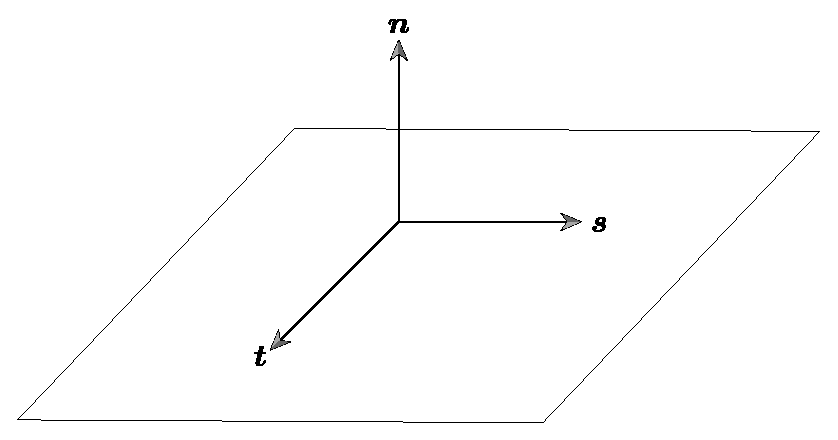
\includegraphics[width=0.7\linewidth]{chap08/BSDFcoordinatesystem.eps}
      \caption{基本BSDF接口设置。着色坐标系由正交基向量$({\bm s},{\bm t},{\bm n})$定义。
            我们将调整这些向量朝向使得它们在该坐标系中沿着$x$、$y$和$z$轴。
            在调用任何BRDF或BTDF方法前,世界空间中的方向向量$\bm \omega$会被
            变换到着色坐标系。}
      \label{fig:8.2}
\end{figure}

着色坐标系也给出了表示球面坐标$(\theta,\varphi)$中方向的坐标系;
角度$\theta$从给定方向测量到$z$轴,$\varphi$是方向投影到$xy$平面后
与$x$轴所成角度。给定该坐标系下的方向向量$\bm\omega$,
很容易计算与法向夹角的余弦等量:
\begin{align*}
      \cos\theta=({\bm n}\cdot{\bm\omega})=((0,0,1)\cdot{\bm\omega})=\omega_z\, .
\end{align*}

我们将提供实用函数来计算这些值和一些有用的变量;
它们的使用有助于阐明BRDF和BTDF的实现。
\begin{lstlisting}
`\initcode{BSDF Inline Functions}{=}\initnext{BSDFInlineFunctions}`
inline `\refvar{Float}{}` `\initvar{CosTheta}{}`(const `\refvar{Vector3f}{}` &w) { return w.z; }
inline `\refvar{Float}{}` `\initvar{Cos2Theta}{}`(const `\refvar{Vector3f}{}` &w) { return w.z * w.z; }
inline `\refvar{Float}{}` `\initvar{AbsCosTheta}{}`(const `\refvar{Vector3f}{}` &w) { return std::abs(w.z); }
\end{lstlisting}

$\sin^2\theta$的值可用三角恒等式$\sin^2\theta+\cos^2\theta=1$算得,
但我们要注意避免取负数的平方根,罕见情况下浮点舍入误差
会让{\ttfamily 1 - \refvar{Cos2Theta}{}(w)}小于零。
\begin{lstlisting}
`\refcode{BSDF Inline Functions}{+=}\lastnext{BSDFInlineFunctions}`
inline `\refvar{Float}{}` `\initvar{Sin2Theta}{}`(const `\refvar{Vector3f}{}` &w) {
    return std::max((`\refvar{Float}{}`)0, (`\refvar{Float}{}`)1 - `\refvar{Cos2Theta}{}`(w));
}
inline `\refvar{Float}{}` `\initvar{SinTheta}{}`(const `\refvar{Vector3f}{}` &w) {
    return std::sqrt(`\refvar{Sin2Theta}{}`(w));
}
\end{lstlisting}

角$\theta$的正切可以由恒等式$\displaystyle\tan\theta=\frac{\sin\theta}{\cos\theta}$计算。
\begin{lstlisting}
`\refcode{BSDF Inline Functions}{+=}\lastnext{BSDFInlineFunctions}`
inline `\refvar{Float}{}` `\initvar{TanTheta}{}`(const `\refvar{Vector3f}{}` &w) {
    return `\refvar{SinTheta}{}`(w) / `\refvar{CosTheta}{}`(w);
}
inline `\refvar{Float}{}` `\initvar{Tan2Theta}{}`(const `\refvar{Vector3f}{}` &w) {
    return `\refvar{Sin2Theta}{}`(w) / `\refvar{Cos2Theta}{}`(w);
}
\end{lstlisting}

我们可以类似地用着色坐标系来简化角$\varphi$的正余弦计算(\reffig{8.3})。
在被着色点的平面内,向量$\bm\omega$的坐标$(x,y)$分别由$r\cos\varphi$和$r\sin\varphi$给出。
半径$r$是$\sin\theta$,所以
\begin{align*}
      \cos\varphi & =\frac{x}{r}=\frac{x}{\sin\theta}\,   \\
      \sin\varphi & =\frac{y}{r}=\frac{y}{\sin\theta}\, .
\end{align*}

\begin{figure}[htbp]
      \centering
      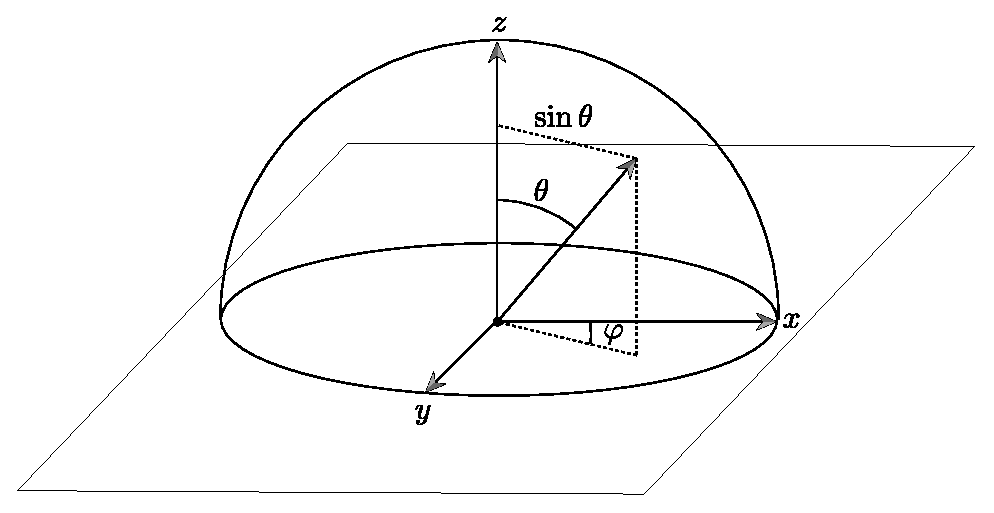
\includegraphics[width=0.7\linewidth]{chap08/BSDFthetaphiangles.eps}
      \caption{$\sin\varphi$和$\cos\varphi$的值可用球面坐标
            方程$x=r\cos\varphi$和$y=r\sin\varphi$算得,其中$r$是虚线的长度,等于$\sin\theta$.}
      \label{fig:8.3}
\end{figure}

\begin{lstlisting}
`\refcode{BSDF Inline Functions}{+=}\lastnext{BSDFInlineFunctions}`
inline `\refvar{Float}{}` `\initvar{CosPhi}{}`(const `\refvar{Vector3f}{}` &w) {
    `\refvar{Float}{}` sinTheta = `\refvar{SinTheta}{}`(w);
    return (sinTheta == 0) ? 1 : `\refvar{Clamp}{}`(w.x / sinTheta, -1, 1);
}
inline `\refvar{Float}{}` `\initvar{SinPhi}{}`(const `\refvar{Vector3f}{}` &w) {
    `\refvar{Float}{}` sinTheta = `\refvar{SinTheta}{}`(w);
    return (sinTheta == 0) ? 0 : `\refvar{Clamp}{}`(w.y / sinTheta, -1, 1);
}
\end{lstlisting}
\begin{lstlisting}
`\refcode{BSDF Inline Functions}{+=}\lastnext{BSDFInlineFunctions}`
inline `\refvar{Float}{}` `\initvar{Cos2Phi}{}`(const `\refvar{Vector3f}{}` &w) {
    return `\refvar{CosPhi}{}`(w) * `\refvar{CosPhi}{}`(w);
}
inline `\refvar{Float}{}` `\initvar{Sin2Phi}{}`(const `\refvar{Vector3f}{}` &w) {
    return `\refvar{SinPhi}{}`(w) * `\refvar{SinPhi}{}`(w);
}
\end{lstlisting}

两个向量在着色坐标系下$\varphi$值间的角$\Delta\varphi$的余弦
可以通过置零两个向量的$z$坐标获得2D向量后再规范化求得。
这两个向量的点积给出了它们夹角的余弦。
为了高效,下面的实现重新排列了项使得只需执行一次平方根运算。
\begin{lstlisting}
`\refcode{BSDF Inline Functions}{+=}\lastnext{BSDFInlineFunctions}`
inline `\refvar{Float}{}` `\initvar{CosDPhi}{}`(const `\refvar{Vector3f}{}` &wa, const `\refvar{Vector3f}{}` &wb) {
    return `\refvar{Clamp}{}`((wa.x * wb.x + wa.y * wb.y) /
                 std::sqrt((wa.x * wa.x + wa.y * wa.y) *
                           (wb.x * wb.x + wb.y * wb.y)), -1, 1);
}
\end{lstlisting}

当阅读本章代码和向pbrt增添BRDF和BTDF时,需要记住一些重要约定和实现细节。
\begin{itemize}
      \item 入射光方向${\bm\omega}_{\mathrm{i}}$和出射查看方向${\bm\omega}_{\mathrm{o}}$都是
            规范化的,且变换到表面的局部坐标系后都是朝外指的。
      \item 按pbrt的约定,曲面法线$\bm n$总是指向物体的“外侧”,这让确定光是进入还是射出透明物体更简单:
            如果入射光方向${\bm\omega}_{\mathrm{i}}$和$\bm n$在同一半球,
            则光在射入;否则光在射出。因此,要记住的一个细节是法线可能相对于
            一个或两个方向向量${\bm\omega}_{\mathrm{i}}$和${\bm\omega}_{\mathrm{o}}$
            在表面的对侧。不像许多其他渲染器那样,pbrt不会翻转法线使其和${\bm\omega}_{\mathrm{o}}$在同侧。
      \item 用于着色的局部坐标系可能并不和来自第\refchap{形状}的例程\refvar{Shape::Intersect}{()}
            返回的坐标系一样;它们在相交和着色间为了达到凹凸贴图等效果可能会被修改。见第\refchap{材质}这类修改的例子。
      \item 最后,BRDF和BTDF的实现不应关心${\bm\omega}_{\mathrm{i}}$和${\bm\omega}_{\mathrm{o}}$是否在同一半球。
            例如,尽管反射BRDF原则上应该检测是否入射方向在表面之上而出射方向在下面并在这种情况下总是不返回反射,
            但这里我们希望反射函数代之以利用其反射模型的合适公式计算和返回反射的光量,
            忽略它们不在同一半球的细节。pbrt中的高层级代码会保证只有反射或透射散射例程会适当求值。
            该约定的价值将在\refsec{BSDF}解释。
\end{itemize}

\section{基本接口}\label{sec:基本接口}
我们将首先定义单个BRDF和BTDF函数的接口。
BRDF和BTDF共享共同的基类\refvar{BxDF}{}。
因为两者都有一样的接口,共享相同的基类减少了重复代码并
允许系统的一些部分和一般的\refvar{BxDF}{}配合而不用区分BRDF和BTDF。
\begin{lstlisting}
`\initcode{BxDF Declarations}{=}\initnext{BxDFDeclarations}`
class `\initvar{BxDF}{}` {
public:
    `\refcode{BxDF Interface}{}`
    `\refcode{BxDF Public Data}{}`
};
\end{lstlisting}

\refsec{BSDF}将要介绍的类\refvar{BSDF}{}持有一系列\refvar{BxDF}{}对象
来一起描述表面上一点的散射。尽管我们把\refvar{BxDF}{}的实现细节隐藏到
反射和透射材质的公共接口后,第\refchap{光传输I:表面反射}到\refchap{光传输III:双向方法}的
一些光传输算法还是需要区分这两个类型。因此,所有\refvar{BxDF}{}都
有成员\refvar{BxDF::type}{}持有来自\refvar{BxDFType}{}的标志。
对于每个\refvar{BxDF}{},该标志应至少有一个置为\refvar[BSDFREFLECTION]{BSDF\_REFLECTION}{}
或\refvar[BSDFTRANSMISSION]{BSDF\_TRANSMISSION}{},且恰有一个漫反射、光泽或镜面标志。
注意没有逆反射标志;这里的分类中逆反射被当作光泽反射。

\begin{lstlisting}
`\initcode{BSDF Declarations}{=}\initnext{BSDFDeclarations}`
enum `\initvar{BxDFType}{}` {
    `\initvar[BSDFREFLECTION]{BSDF\_REFLECTION}{}` = 1 << 0,
    `\initvar[BSDFTRANSMISSION]{BSDF\_TRANSMISSION}{}` = 1 << 1,
    `\initvar[BSDFDIFFUSE]{BSDF\_DIFFUSE}{}` = 1 << 2,
    `\initvar[BSDFGLOSSY]{BSDF\_GLOSSY}{}` = 1 << 3,
    `\initvar[BSDFSPECULAR]{BSDF\_SPECULAR}{}` = 1 << 4,
    `\initvar[BSDFALL]{BSDF\_ALL}{}` = BSDF_DIFFUSE | BSDF_GLOSSY | BSDF_SPECULAR |
                        BSDF_REFLECTION | BSDF_TRANSMISSION,
};
\end{lstlisting}

\begin{lstlisting}
`\initcode{BxDF Interface}{=}\initnext{BxDFInterface}`
`\refvar{BxDF}{}`(`\refvar{BxDFType}{}` type) : `\refvar[BxDF::type]{type}{}`(type) { }
\end{lstlisting}

\begin{lstlisting}
`\initcode{BxDF Public Data}{=}`
const `\refvar{BxDFType}{}` `\initvar[BxDF::type]{type}{}`;
\end{lstlisting}

实用方法\refvar{MatchesFlags}{()}确定\refvar{BxDF}{}是否匹配用户提供的类型标志:
\begin{lstlisting}
`\refcode{BxDF Interface}{+=}\lastnext{BxDFInterface}`
bool `\initvar{MatchesFlags}{}`(`\refvar{BxDFType}{}` t) const {
    return (`\refvar[BxDF::type]{type}{}` & t) == `\refvar[BxDF::type]{type}{}`;
}
\end{lstlisting}

\refvar{BxDF}{}提供的关键方法是\refvar{BxDF::f}{()}。
它为给定的方向对返回分布函数的值。该接口隐式假设了不同波长的光是解耦的——
某一波长的能量不会反射成不同波长。通过作出该假设,反射函数的效应可以直接用\refvar{Spectrum}{}表示。
支持该假设不成立的荧光材料则要求该方法返回一个$n\times n$矩阵以编码光谱样本间的能量转化
(其中$n$是\refvar{Spectrum}{}表示中的样本数量)。
\begin{lstlisting}
`\refcode{BxDF Interface}{+=}\lastnext{BxDFInterface}`
virtual `\refvar{Spectrum}{}` `\initvar[BxDF::f]{f}{}`(const `\refvar{Vector3f}{}` &wo, const `\refvar{Vector3f}{}` &wi) const = 0;
\end{lstlisting}

不是所有\refvar{BxDF}{}都能用方法\refvar[BxDF::f]{f}{()}求值。
例如,像镜子、玻璃或水那样的完美镜面物体只把来自单个入射方向的光朝单个出射方向散射。
这样的\refvar{BxDF}{}最好用$\delta$分布描述,即除了光散射的单个方向外都取零。
pbrt中这些\refvar{BxDF}{}需要特殊处理,所以我们也会提供方法\refvar[BxDF::Samplef]{BxDF::Sample\_f}{()}。
该方法既能用于处理由$\delta$分布描述的散射,
也能从散射光有多个方向的\refvar{BxDF}{}中随机采样方向;
第二种应用将在\refsec{采样反射函数}中讨论蒙特卡罗BSDF采样时解释。

\refvar[BxDF::Samplef]{BxDF::Sample\_f}{()}计算给定出射方向${\bm\omega}_{\mathrm{o}}$的
入射光方向${\bm\omega}_{\mathrm{i}}$并为这对方向返回\refvar{BxDF}{}的值。
对于$\delta$分布,\refvar{BxDF}{}有必要这样选择入射光方向,因为调用者
无法生成合适的方向${\bm\omega}_{\mathrm{i}}$
\footnote{反射函数中的$\delta$分布对于光传输算法有一些额外微妙的影响。
    \refsub{镜面反射与透射}和\refsub{被积函数中的delta分布}详细描述了该问题。}。
$\delta$分布的\refvar{BxDF}{}不需要参数{\ttfamily sample}和{\ttfamily pdf},
所以它们会在后面的\refsec{采样反射函数}解释,到时我们将为非镜面反射函数提供该方法的实现。
\begin{lstlisting}
`\refcode{BxDF Interface}{+=}\lastnext{BxDFInterface}`
virtual `\refvar{Spectrum}{}` `\initvar[BxDF::Samplef]{Sample\_f}{}`(const `\refvar{Vector3f}{}` &wo, `\refvar{Vector3f}{}` *wi,
    const `\refvar{Point2f}{}` &sample, `\refvar{Float}{}` *pdf,
    `\refvar{BxDFType}{}` *sampledType = nullptr) const;
\end{lstlisting}

\subsection{反射}\label{sub:反射}
将4D的BRDF或BTDF的表现聚合起来定义为一对方向上的函数,
并将其简化为单个方向上的2D函数甚至是描述其整体散射表现的常数值很有用。

\keyindex{半球定向反射率}{hemispherical-directional reflectance}{}是
一个2D函数,它给出了半球上常量照明于给定方向上的反射率,
或者等价地,因来自给定方向的光而在半球上的总反射率
\footnote{这两个量相等的事实源自反射函数的互易性。BTDF通常不互易;见\refsub{非对称散射}。}。
它定义为
\begin{align}
    \label{eq:8.1}
    \rho_{\mathrm{hd}}({\bm\omega}_{\mathrm{o}})=\int\limits_{H^2({\bm n})}{f_{\mathrm{r}}({\bm p},{\bm \omega}_\mathrm{o},{\bm \omega}_\mathrm{i})|\cos{\theta_{\mathrm{i}}}|\mathrm{d}{\bm \omega}_\mathrm{i}}\, .
\end{align}

方法\refvar{BxDF::rho}{()}计算反射函数$\rho_{\mathrm{hd}}$.
一些\refvar{BxDF}{}能解析地计算该值,然而大部分用蒙特卡罗积分来计算其近似值。
对于那些\refvar{BxDF}{},参数{\ttfamily nSamples}和{\ttfamily samples}供
蒙特卡罗算法的实现使用;它们将在\refsub{应用:估计反射率}解释。
\begin{lstlisting}
`\refcode{BxDF Interface}{+=}\lastnext{BxDFInterface}`
virtual `\refvar{Spectrum}{}` `\initvar[BxDF::rho]{rho}{}`(const `\refvar{Vector3f}{}` &wo, int nSamples,
                     const `\refvar{Point2f}{}` *samples) const;
\end{lstlisting}

表面的\keyindex{半球半球反射率}{hemispherical-hemispherical reflectance}{}记为$\rho_{\mathrm{hh}}$,
该光谱值给出了当各方向入射光相同时表面反射的入射光比例。它是
\begin{align*}
    \rho_{\mathrm{hh}}=\frac{1}{\pi}\int\limits_{H^2({\bm n})}\int\limits_{H^2({\bm n})}f_{\mathrm{r}}({\bm p},{\bm \omega}_\mathrm{o},{\bm \omega}_\mathrm{i})|\cos{\theta_{\mathrm{o}}}\cos{\theta_{\mathrm{i}}}|\mathrm{d}{\bm \omega}_\mathrm{o}\mathrm{d}{\bm \omega}_\mathrm{i}\, .
\end{align*}

如果不提供方向${\bm\omega}_\mathrm{o}$,则方法\refvar[BxDF::rho2]{BxDF::rho}{()}计算$\rho_{\mathrm{hh}}$.
剩下的参数又是在需要时用于计算$\rho_{\mathrm{hh}}$值的蒙特卡罗估计。
\begin{lstlisting}
`\refcode{BxDF Interface}{+=}\lastcode{BxDFInterface}`
virtual `\refvar{Spectrum}{}` `\initvar[BxDF::rho2]{rho}{}`(int nSamples, const `\refvar{Point2f}{}` *samples1,
                     const `\refvar{Point2f}{}` *samples2) const;
\end{lstlisting}

\subsection{BxDF缩放适配器}\label{sub:BxDF缩放适配器}
取一个给定的\refvar{BxDF}{}并用一个\refvar{Spectrum}{}值
缩放它的作用也很有用。\refvar{ScaledBxDF}{}
封装器持有一个\refvar{BxDF}{*}和\refvar{Spectrum}{}并实现其功能。
该类由\refvar{MixMaterial}{}(定义于\refsub{混合材料})使用,
它基于另两种材料的加权和创建\refvar{BSDF}{}。
\begin{lstlisting}
`\refcode{BxDF Declarations}{+=}\lastnext{BxDFDeclarations}`
class `\initvar{ScaledBxDF}{}` : public `\refvar{BxDF}{}` {
public:
    `\refcode{ScaledBxDF Public Methods}{}`
private:
    `\refvar{BxDF}{}` *`\initvar[ScaledBxDF::bxdf]{bxdf}{}`;
    `\refvar{Spectrum}{}` `\initvar[ScaledBxDF::scale]{scale}{}`;
};
\end{lstlisting}
\begin{lstlisting}
`\initcode{ScaledBxDF Public Methods}{=}`
`\refvar{ScaledBxDF}{}`(`\refvar{BxDF}{}` *bxdf, const `\refvar{Spectrum}{}` &scale)
    : `\refvar{BxDF}{}`(`\refvar{BxDFType}{}`(bxdf->`\refvar[BxDF::type]{type}{}`)), `\refvar[ScaledBxDF::bxdf]{bxdf}{}`(bxdf), `\refvar[ScaledBxDF::scale]{scale}{}`(scale) {
}
\end{lstlisting}

\refvar{ScaledBxDF}{}的方法实现很简单;我们这里只介绍\refvar[ScaledBxDF::f]{f}{()}。
\begin{lstlisting}
`\initcode{BxDF Method Definitions}{=}\initnext{BxDFMethodDefinitions}`
`\refvar{Spectrum}{}` `\refvar{ScaledBxDF}{}`::`\initvar[ScaledBxDF::f]{f}{}`(const `\refvar{Vector3f}{}` &wo, const `\refvar{Vector3f}{}` &wi) const {
    return `\refvar[ScaledBxDF::scale]{scale}{}` * `\refvar[ScaledBxDF::bxdf]{bxdf}{}`->`\refvar[BxDF::f]{f}{}`(wo, wi);
}
\end{lstlisting}

\section{镜面反射与透射}\label{sec:镜面反射与透射}

绝对光滑表面上光的特性较容易用物理和几何光学模型分析刻画。
这些表面展现出入射光的完美镜像反射和透射;
对于给定的方向${\bm\omega}_{\mathrm{i}}$,
所有光都散射到单个出射方向${\bm\omega}_{\mathrm{o}}$.
对于镜面反射,该出射方向和法线所成角与入射方向相同:
\begin{align*}
    \theta_{\mathrm{i}}=\theta_{\mathrm{o}}\, ,
\end{align*}
且其中$\varphi_{\mathrm{o}}=\varphi_{\mathrm{i}}+\pi$.
对于透射,我们也有$\varphi_{\mathrm{o}}=\varphi_{\mathrm{i}}+\pi$,
且出射方向$\theta_{\mathrm{t}}$由斯涅尔定律给出,
它将折射方向与曲面法线$\bm n$的夹角$\theta_{\mathrm{t}}$与
入射光线与曲面法线$\bm n$的夹角$\theta_{\mathrm{i}}$联系起来
(本章末的习题之一是用光学的费马原理推导斯涅尔定律)。
斯涅尔定律基于入射光线所在介质的\keyindex{折射率}{index of refraction}{}和
要进入的介质的折射率。折射率描述了光在特定介质中相比在真空中传播要慢多少。
我们用希腊字母$\eta$表示折射率,读作“eta”。斯涅尔定律是
\begin{align}
    \label{eq:8.2}
    \eta_{\mathrm{i}}\sin\theta_{\mathrm{i}}=\eta_{\mathrm{t}}\sin\theta_{\mathrm{t}}\, .
\end{align}

通常,折射率随波长变化。因此,在两种不同介质界面上入射光通常散射到多个方向,
该效应称为\keyindex{色散}{dispersion}{}。
当入射白光被棱镜分出光谱成分时可以观察到该效应。
图形学中的通行做法是忽略该波长依赖性,
因为该效应通常对视觉准确性并不关键且忽略它能极大简化光传输计算。
可选地,可以在有色散物体的环境中追踪多束光路(例如一系列离散波长)。
第\refchap{光传输I:表面反射}末的“扩展阅读”一节有关于该话题的更多信息指引。
\begin{figure}[htbp]
    \centering
    \subfloat[镜面反射]{\includegraphics[width=0.75\linewidth]{chap08/dragon-specular-reflect.png}\label{fig:8.4.1}}\\
    \subfloat[镜面透射]{\includegraphics[width=0.75\linewidth]{chap08/dragon-specular-transmit.png}\label{fig:8.4.2}}
    \caption{用(1)完美镜面反射和(2)完美镜面折射渲染的龙模型。图像(2)排除了
        内外反射的影响;导致的能量损失产生了显眼的暗区(感谢Christian Schüller提供模型)。}
    \label{fig:8.4}
\end{figure}

\reffig{8.4}展示了完美镜面反射和透射的效果。

\subsection{菲涅尔反射率}\label{sub:菲涅尔反射率}
除了反射和透射方向,还有必要计算反射或透射的入射光占比。
为了物理上准确反射或折射,该项依赖于方向,而不能用每个表面的缩放常数表征。
\keyindex{菲涅耳方程}{Fresnel equations}{}
\sidenote{译者注:得名于法国物理学家奥古斯丁·菲涅耳(Augustin-Jean Fresnel)。}描述了
表面上反射光的量;它们是麦克斯韦方程在光滑表面上的解。

给定折射率和入射光与曲面法线所成角度,菲涅耳方程
指定了材料对两种不同偏振状态的入射照明相应的反射率。
因为偏振的视觉效果在大多数环境下是受限的,
所以在pbrt中我们将作出光是无偏振的常用假设;
即光波是随机朝向的。有了该简化假设,菲涅尔反射率就是
平行和垂直偏振项的均方。

此刻有必要指出几个重要材料类别的差异:
\begin{enumerate}
    \item 第一类是\keyindex{介电质}{dielectric}{},
          是不会导电的材料。它们有实数值的折射率(通常在范围1-3内)且
          透射\footnote{注意介电质可能充满能吸收大部分或所有透射光的粒子(例如石油)。
              像水那样的介电质也能通过添加离子使之导电而变成电解质溶液。
              这两方面都和材料本身划分为介电质或导体无关。}一部分入射照明。
          介电质的例子有玻璃、矿油、水和空气。
    \item 第二类组成是\keyindex{导体}{conductor}{}例如金属。
          价电子可以自由地在原子晶格中移动,允许电流从一个地方流到另一处。
          当导体受到电磁辐射例如可见光时,这一基本的原子属性就会转化为完全不同的特性:
          该材料是不透明的并反射回大部分照明。一部分光也透射进导体内部并被迅速吸收:
          总吸收通常发生在材料表面0.1$\mu\mathrm{m}$内,因此只有极薄的金属膜才能透射足够的光量。
          我们在pbrt中忽略该效应而只建模导体的反射部分。与介电质相反,
          导体有复数值的折射率$\bar{\eta}=\eta+\mathrm{i}k$.
    \item \keyindex{半导体}{semiconductor}{}例如硅或锗是本书中我们不予考虑的第三类。
\end{enumerate}

导体和介电质都由同一组菲涅尔方程表征。
尽管如此,我们更喜欢为介电质创建特殊的求值函数,
这样当折射率保证为实数值时,这些方程会取特别简单的形式。

\begin{table}[htbp]
    \centering
    \begin{tabular}{ll}
        \toprule
        \textbf{介质}  & \textbf{折射率}$\eta$ \\
        \midrule
        真空           & 1.0                   \\
        海平面上的空气 & 1.00029               \\
        冰             & 1.31                  \\
        水(20℃)      & 1.333                 \\
        熔融石英       & 1.46                  \\
        玻璃           & 1.5-1.6               \\
        蓝宝石         & 1.77                  \\
        钻石           & 2.42                  \\
        \bottomrule
    \end{tabular}
    \caption{各种物体的折射率,给出了光在真空中的速度与
        光在介质中的速度的比值。它们通常是与波长相关的量;
        这些值是在可见波长上的均值。}
    \label{tab:8.1}
\end{table}

为了计算两种介电质界面处的菲涅尔反射率,我们
需要知道这两种介质的折射率。\reftab{8.1}有许多介电质的折射率。
介电质的菲涅尔反射率公式是
\begin{align*}
    r_{\parallel} & =\frac{\eta_{\mathrm{t}}\cos\theta_{\mathrm{i}}-\eta_{\mathrm{i}}\cos\theta_{\mathrm{t}}}{\eta_{\mathrm{t}}\cos\theta_{\mathrm{i}}+\eta_{\mathrm{i}}\cos\theta_{\mathrm{t}}}\, , \\
    r_{\perp}     & =\frac{\eta_{\mathrm{i}}\cos\theta_{\mathrm{i}}-\eta_{\mathrm{t}}\cos\theta_{\mathrm{t}}}{\eta_{\mathrm{i}}\cos\theta_{\mathrm{i}}+\eta_{\mathrm{t}}\cos\theta_{\mathrm{t}}}\, ,
\end{align*}
其中$r_{\parallel}$是平行偏振光的菲涅尔反射率,
$r_{\perp}$是垂直偏振光的反射率,$eta_{\mathrm{i}}$和$\eta_{\mathrm{t}}$是
入射和透射介质的折射率,$\bm\omega_{\mathrm{i}}$和$\bm\omega_{\mathrm{t}}$是
入射和透射方向。$\bm\omega_{\mathrm{t}}$由斯涅尔定律算出(见\refsub{镜面透射})。

余弦项应该大于或等于零;出于计算这些值的目的,
当计算$\cos\theta_{\mathrm{i}}$和$\cos\theta_{\mathrm{t}}$时,
几何法线应该分别翻转到和$\bm\omega_{\mathrm{i}}$或$\bm\omega_{\mathrm{t}}$同侧。

对于非偏振光,菲涅尔反射率是
\begin{align*}
    F_{\mathrm{r}}=\frac{1}{2}(r_{\parallel}^2+r_{\perp}^2)\, .
\end{align*}

因为能量守恒,介电质传输的能量为$1-F_{\mathrm{r}}$.

函数\refvar{FrDielectric}{()}为介电质材料和非偏振光计算菲涅尔反射率公式。
量$\cos\theta_{\mathrm{i}}$作为参数{\ttfamily cosThetaI}传入。
\begin{lstlisting}
`\initcode{BxDF Utility Functions}{=}`
`\refvar{Float}{}` `\initvar{FrDielectric}{}`(`\refvar{Float}{}` cosThetaI, `\refvar{Float}{}` etaI, `\refvar{Float}{}` etaT) {
    cosThetaI = `\refvar{Clamp}{}`(cosThetaI, -1, 1);
    `\refcode{Potentially swap indices of refraction}{}`
    `\refcode{Compute cosThetaT using Snell's law}{}`
    `\refvar{Float}{}` Rparl = ((etaT * cosThetaI) - (etaI * cosThetaT)) /
                  ((etaT * cosThetaI) + (etaI * cosThetaT));
    `\refvar{Float}{}` Rperp = ((etaI * cosThetaI) - (etaT * cosThetaT)) /
                  ((etaI * cosThetaI) + (etaT * cosThetaT));
    return (Rparl * Rparl + Rperp * Rperp) / 2;
}
\end{lstlisting}

为了求得折射角的余弦{\ttfamily cosThetaT},
首先需要确定入射方向是在介质的外面还是里面,这样才能恰当解释两个折射率。

入射角余弦的符号表明了入射光在介质的哪一侧(\reffig{8.5})。
如果余弦在0到1间,则光线在外侧,如果在-1到0间,则光线在内侧。
调整参数{\ttfamily etaI}和{\ttfamily etaT}使得{\ttfamily etaI}
是入射介质的折射率,这样保证了{\ttfamily cosThetaI}非负。

\begin{figure}[htbp]
    \centering
    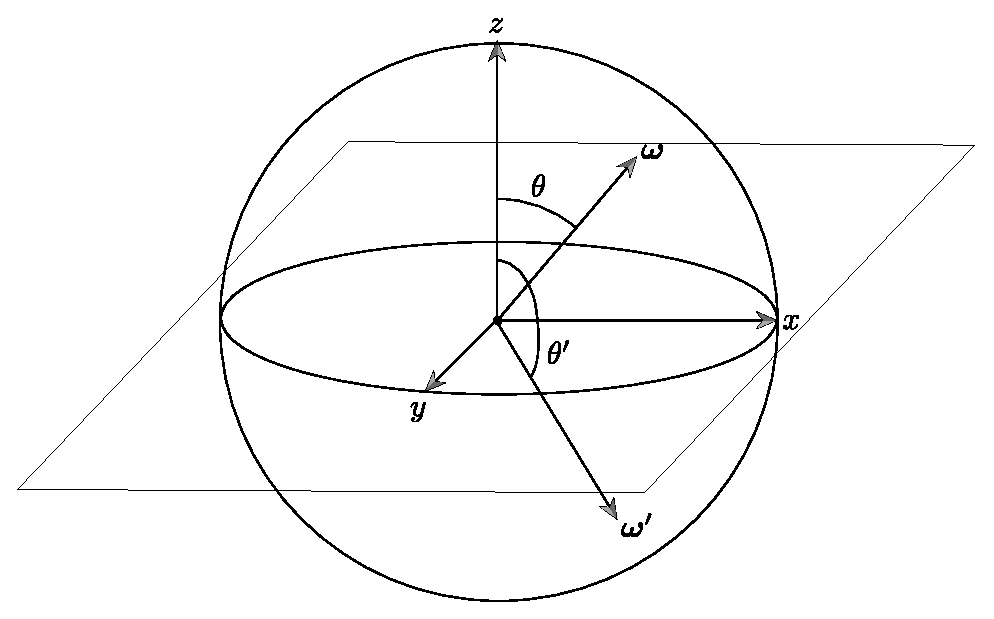
\includegraphics[width=0.7\linewidth]{chap08/BSDFanglegivesinout.eps}
    \caption{方向$\bm\omega$和几何曲面法线间夹角$\theta$的余弦
        表明方向是指向表面外侧(和法线在同一半球)还是表面内侧。
        在标准反射坐标系中,该测试只要求检查方向向量的$z$分量。
        这里,$\bm\omega$在上半球,取正值余弦,而${\bm\omega}'$在下半球。}
    \label{fig:8.5}
\end{figure}

\begin{lstlisting}
`\initcode{Potentially swap indices of refraction}{=}`
bool entering = cosThetaI > 0.f;
if (!entering) {
    std::swap(etaI, etaT);
    cosThetaI = std::abs(cosThetaI);
}
\end{lstlisting}

一旦确定折射率,我们就能用斯涅尔定律(\refeq{8.2})计算
透射方向和曲面法线夹角的正弦$\sin\theta_{\mathrm{t}}$.
最后,用恒等式$\sin^2\theta+\cos^2\theta=1$求得该角的余弦。
\begin{lstlisting}
`\initcode{Compute cosThetaT using Snell's law}{=}`
`\refvar{Float}{}` sinThetaI = std::sqrt(std::max((`\refvar{Float}{}`)0,
                                     1 - cosThetaI * cosThetaI));
`\refvar{Float}{}` sinThetaT = etaI / etaT * sinThetaI;
`\refcode{Handle total internal reflection}{}`
`\refvar{Float}{}` cosThetaT = std::sqrt(std::max((`\refvar{Float}{}`)0,
                                     1 - sinThetaT * sinThetaT));
\end{lstlisting}

当从一种介质传播到另一种折射率更低的介质时,入射角接近掠角的光不能进入另一介质。
发生该现象的最大角称为\keyindex{临界角}{critical angle}{};
当$\theta_{\mathrm{i}}$大于临界角时,发生\keyindex{全内反射}{total internal reflection}{reflection反射},
所有光都被反射。这里通过$\sin\theta_{\mathrm{t}}$大于1检测到该情况;
此时不需要菲涅尔方程。
\begin{lstlisting}
`\initcode{Handle total internal reflection}{=}`
if (sinThetaT >= 1)
    return 1;
\end{lstlisting}

我们现在聚焦一般情况下的复数折射率$\bar{\eta}=\eta+\mathrm{i}k$,
其中一些入射光被材料部分吸收并变为热量。
除了实部,一般菲涅尔公式现在也依赖于虚部$k$,
称为\keyindex{吸收系数}{absorption coefficient}{}。

\reffig{8.6}展示了金的折射率和吸收系数图示。两者都是与波长相关的量。
pbrt发行版中目录{\ttfamily scenes/spds/metals}下有各种金属的$\eta$与$k$与波长相关的数据。
下章的\reffig{9.4}展示了用金属材料渲染的模型。
\begin{figure}[htbp]
    \centering
    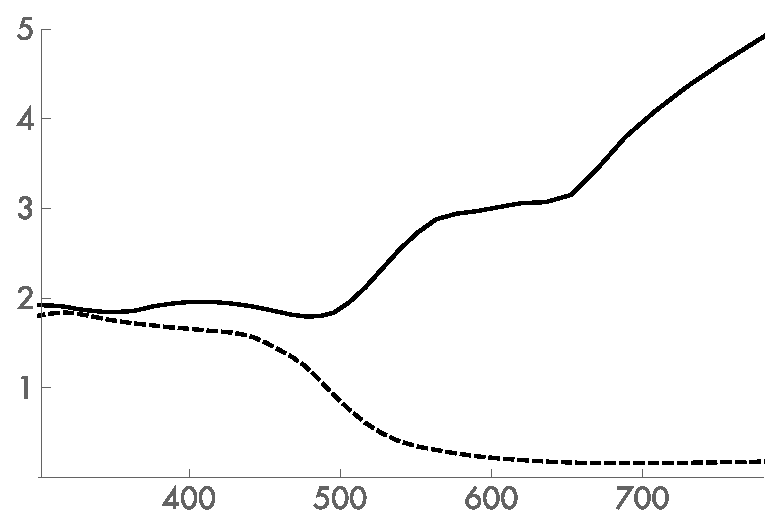
\includegraphics[width=0.7\linewidth]{chap08/au-k-eta.eps}
    \caption{金的吸收系数和折射率。该图展示了金的吸收系数$k$(实线)
        和折射率$\eta$(虚线)随光谱变化的值,横轴是波长,单位纳米。}
    \label{fig:8.6}
\end{figure}

导体和介电质界面处的菲涅尔反射率是
\begin{align}
    \label{eq:8.3}
    r_{\perp}     & =\frac{a^2+b^2-2a\cos\theta+\cos^2\theta}{a^2+b^2+2a\cos\theta+\cos^2\theta}\, ,\nonumber                                                     \\
    r_{\parallel} & =r_{\perp}\frac{(a^2+b^2)\cos^2\theta-2a\cos\theta\sin^2\theta+\sin^4\theta}{(a^2+b^2)\cos^2\theta+2a\cos\theta\sin^2\theta+\sin^4\theta}\, ,
\end{align}
其中
\begin{align*}
    a^2+b^2=\sqrt{(\eta^2-k^2-\sin^2\theta)^2+4\eta^2k^2}\, ,
\end{align*}
且$\displaystyle\eta+\mathrm{i}k=\frac{\bar{\eta_\mathrm{t}}}{\bar{\eta_\mathrm{i}}}$是
用复数除法算出的相对折射率。然而,通常$\bar{\eta_\mathrm{i}}$是介电质的
所以可以替代使用普通的实数除法。

该计算由函数\refvar{FrConductor}{()}实现
\footnote{注意这稍微用词不当,因为函数在技术上包含了介电质$k=0$的情况。
    也就是说,我们选这个名称是为了表明该函数应只用于处理导体,
    因为它比求\refvar{FrDielectric}{()}的开销更大。};
该实现直接对应\refeq{8.3}所以这里不介绍了。
\begin{lstlisting}
`\initcode{Reflection Declarations}{=}`
`\refvar{Spectrum}{}` `\initvar{FrConductor}{}`(`\refvar{Float}{}` cosThetaI, const `\refvar{Spectrum}{}` &etaI,
    const `\refvar{Spectrum}{}` &etaT, const `\refvar{Spectrum}{}` &k);
\end{lstlisting}

为了方便,我们定义抽象类\refvar{Fresnel}{}以提供接口计算菲涅尔反射系数。
用该接口的实现帮助简化后续可能需要支持两种形式的BRDF实现。
\begin{lstlisting}
`\refcode{BxDF Declarations}{+=}\lastnext{BxDFDeclarations}`
class `\initvar{Fresnel}{}` {
public:
    `\refcode{Fresnel Interface}{}`
};
\end{lstlisting}

\refvar{Fresnel}{}接口提供的唯一函数是\refvar{Fresnel::Evaluate}{()}。
给定入射方向和曲面法线夹角的余弦,它返回表面反射的光量。
\begin{lstlisting}
`\initcode{Fresnel Interface}{=}`
virtual `\refvar{Spectrum}{}` `\initvar[Fresnel::Evaluate]{Evaluate}{}`(`\refvar{Float}{}` cosI) const = 0;
\end{lstlisting}

\subsubsection*{菲涅尔导体}
\refvar{FresnelConductor}{}为导体实现该接口。
\begin{lstlisting}
`\refcode{BxDF Declarations}{+=}\lastnext{BxDFDeclarations}`
class `\initvar{FresnelConductor}{}` : public `\refvar{Fresnel}{}` {
public:
    `\refcode{FresnelConductor Public Methods}{}`
private:
    `\refvar{Spectrum}{}` `\initvar[FresnelConductor::etaI]{etaI}{}`, `\initvar[FresnelConductor::etaT]{etaT}{}`, `\initvar[FresnelConductor::k]{k}{}`;
};
\end{lstlisting}

其构造函数存有给定的折射率$\eta$和吸收系数$k$.
\begin{lstlisting}
`\initcode{FresnelConductor Public Methods}{=}`
`\refvar{FresnelConductor}{}`(const `\refvar{Spectrum}{}` &etaI, const `\refvar{Spectrum}{}` &etaT,
    const `\refvar{Spectrum}{}` &k) : `\refvar[FresnelConductor::etaI]{etaI}{}`(etaI), `\refvar[FresnelConductor::etaT]{etaT}{}`(), `\refvar[FresnelConductor::k]{k}{}`(k) { }
\end{lstlisting}

\refvar{FresnelConductor}{}的求值例程也很简单;它只需调用之前定义的函数
\refvar{FrConductor}{()}。注意在调用\refvar{FrConductor}{()}
前{\ttfamily cosThetaI}要取绝对值,因为\refvar{FrConductor}{()}
要求该余弦是在法线和${\bm\omega}_{\mathrm{i}}$在表面的同一侧时测出的,
或者等价地,应该用$\cos\theta_{\mathrm{i}}$的绝对值。
\begin{lstlisting}
`\refcode{BxDF Method Definitions}{+=}\lastnext{BxDFMethodDefinitions}`
`\refvar{Spectrum}{}` `\refvar{FresnelConductor}{}`::`\initvar[FresnelConductor::Evaluate]{Evaluate}{}`(`\refvar{Float}{}` cosThetaI) const {
    return `\refvar{FrConductor}{}`(std::abs(cosThetaI), `\refvar[FresnelConductor::etaI]{etaI}{}`, `\refvar[FresnelConductor::etaT]{etaT}{}`, `\refvar[FresnelConductor::k]{k}{}`);
}
\end{lstlisting}

\subsubsection*{菲涅尔介电质}
\refvar{FresnelDielectric}{}类似地为介电质材料实现了\refvar{Fresnel}{}接口。
\begin{lstlisting}
`\refcode{BxDF Declarations}{+=}\lastnext{BxDFDeclarations}`
class `\initvar{FresnelDielectric}{}` : public `\refvar{Fresnel}{}` {
public:
    `\refcode{FresnelDielectric Public Methods}{}`
private:
    `\refvar{Float}{}` `\initvar[FresnelDielectric::etaI]{etaI}{}`, `\initvar[FresnelDielectric::etaT]{etaT}{}`;
};
\end{lstlisting}

其构造函数存有表面内外侧的折射率。
\begin{lstlisting}
`\initcode{FresnelDielectric Public Methods}{=}`
`\refvar{FresnelDielectric}{}`(`\refvar{Float}{}` etaI, `\refvar{Float}{}` etaT) : `\refvar[FresnelDielectric::etaI]{etaI}{}`(etaI), `\refvar[FresnelDielectric::etaT]{etaT}{}`(etaT) { }
\end{lstlisting}

\refvar{FresnelDielectric}{}的求值例程类似地调用\refvar{FrDielectric}{()}。
\begin{lstlisting}
`\refcode{BxDF Method Definitions}{+=}\lastnext{BxDFMethodDefinitions}`
`\refvar{Spectrum}{}` `\refvar{FresnelDielectric}{}`::`\initvar[FresnelDielectric::Evaluate]{Evaluate}{}`(`\refvar{Float}{}` cosThetaI) const {
    return `\refvar{FrDielectric}{}`(cosThetaI, `\refvar[FresnelDielectric::etaI]{etaI}{}`, `\refvar[FresnelDielectric::etaT]{etaT}{}`);
}
\end{lstlisting}

\subsubsection*{特殊菲涅尔接口}
\refvar{Fresnel}{}接口的实现\refvar{FresnelNoOp}{}对所有入射方向返回100\%反射率。
尽管这在物理上不可实现,但这是可用的方便能力。
\begin{lstlisting}
`\refcode{BxDF Declarations}{+=}\lastnext{BxDFDeclarations}`
class `\initvar{FresnelNoOp}{}` : public `\refvar{Fresnel}{}` {
public:
    `\refvar{Spectrum}{}` `\initvar[FresnelNoOp::Evaluate]{Evaluate}{}`(`\refvar{Float}{}`) const { return `\refvar{Spectrum}{}`(1.); }
};
\end{lstlisting}

\subsection{镜面反射}\label{sub:镜面反射}
我们现在可以实现类\refvar{SpecularReflection}{},
它用菲涅尔接口计算反射光的占比,描述了物理可实现的镜面反射。
首先,我们将推导描述镜面反射的BRDF。
既然菲涅尔方程给出了反射光的比例$F_{\mathrm{r}}({\bm\omega})$,
那么我们需要这样的BRDF
\begin{align*}
    L_{\mathrm{o}}({\bm\omega}_{\mathrm{o}})=\int{f_{\mathrm{r}}({\bm\omega}_{\mathrm{o}},{\bm\omega}_{\mathrm{i}})L_{\mathrm{i}}({\bm\omega}_{\mathrm{i}})|\cos\theta_{\mathrm{i}}|\mathrm{d}{\bm\omega}_{\mathrm{i}}}=F_{\mathrm{r}}({\bm\omega}_{\mathrm{r}})L_{\mathrm{i}}({\bm\omega}_{\mathrm{r}})\, ,
\end{align*}
其中${\bm\omega}_{\mathrm{r}}=R({\bm\omega}_{\mathrm{o}},{\bm n})$是由${\bm\omega}_{\mathrm{o}}$关于
曲面法线$\bm n$反射的镜面反射向量(回想对于镜面反射有$\theta_{\mathrm{r}}=\theta_{\mathrm{o}}$,
因此$F_{\mathrm{r}}({\bm\omega}_{\mathrm{o}})=F_{\mathrm{r}}({\bm\omega}_{\mathrm{r}})$)。

此类BRDF可用狄拉克$\delta$分布构造。
回顾\refsec{采样理论}中$\delta$分布有个好用的性质
\begin{align}\label{eq:8.4}
    \int{f(x)\delta(x-x_0)\mathrm{d}x}=f(x_0)\, .
\end{align}
然而相比于标准函数,$\delta$分布需要特殊处理。
特别地,对有$\delta$分布的积分求数值积分必须显式考虑$\delta$分布。
考虑\refeq{8.4}中的积分:如果我们尝试用梯形法则或
其他一些数值积分技术计算它,则按$\delta$分布的定义,
在任意取值点$x_i$处$\delta(x_i)$为非零值的概率都为零。
确切地说,我们必须允许$\delta$分布自己确定取值点。
我们将在来自特殊\refvar{BxDF}{}的光传输积分以及
第\refchap{光源}的一些光源中遇到$\delta$分布。

直觉上,我们想让镜面反射BRDF在完美反射方向以外任何地方都取零,
这暗示了要用$\delta$分布。首先可能想到的是用$\delta$函数
把入射方向限制到镜面反射方向${\bm\omega}_{\mathrm{r}}$.
这样得到BRDF
\begin{align*}
    f_{\mathrm{r}}({\bm\omega}_{\mathrm{o}},{\bm\omega}_{\mathrm{i}})=\delta_{\mathrm{r}}({\bm\omega}_{\mathrm{i}}-{\bm\omega}_{\mathrm{r}})F_{\mathrm{r}}({\bm\omega}_{\mathrm{i}})\, .
\end{align*}

尽管这看起来很诱人,但把它代入散射方程\refeq{5.9}就暴露了问题:
\begin{align*}
    L_{\mathrm{o}}({\bm\omega}_{\mathrm{o}}) & =\int{\delta_{\mathrm{r}}({\bm\omega}_{\mathrm{i}}-{\bm\omega}_{\mathrm{r}})F_{\mathrm{r}}({\bm\omega}_{\mathrm{i}})}L_{\mathrm{i}}({\bm\omega}_{\mathrm{i}})|\cos\theta_{\mathrm{i}}|\mathrm{d}{\bm\omega}_{\mathrm{i}} \\
                                             & =F_{\mathrm{r}}({\bm\omega}_{\mathrm{r}})L_{\mathrm{i}}({\bm\omega}_{\mathrm{r}})|\cos\theta_{\mathrm{r}}|\, .
\end{align*}
这是错的,因为它含有额外因子$\cos\theta_{\mathrm{r}}$.
然而,我们可以把该因子分解以求得完美镜面反射正确的BRDF:
\begin{align*}
    f_\mathrm{r}({\bm p},{\bm \omega}_\mathrm{o},{\bm \omega}_\mathrm{i})=F_{\mathrm{r}}({\bm\omega}_{\mathrm{r}})\frac{\delta_{\mathrm{r}}({\bm\omega}_{\mathrm{i}}-{\bm\omega}_{\mathrm{r}})}{|\cos\theta_{\mathrm{r}|}}\, ,
\end{align*}
\begin{lstlisting}
`\refcode{BxDF Declarations}{+=}\lastnext{BxDFDeclarations}`
class `\initvar{SpecularReflection}{}` : public `\refvar{BxDF}{}` {
public:
    `\refcode{SpecularReflection Public Methods}{}`
private:
    `\refcode{SpecularReflection Private Data}{}`
};
\end{lstlisting}

\refvar{SpecularReflection}{}的构造函数接收用于缩放反射颜色的\refvar{Spectrum}{}和
描述介电质或导体菲涅尔性质的\refvar{Fresnel}{}对象指针。
\begin{lstlisting}
`\initcode{SpecularReflection Public Methods}{=}\initnext{SpecularReflectionPublicMethods}`
`\refvar{SpecularReflection}{}`(const `\refvar{Spectrum}{}` &R, `\refvar{Fresnel}{}` *fresnel) 
    : `\refvar{BxDF}{}`(`\refvar{BxDFType}{}`(`\refvar[BSDFREFLECTION]{BSDF\_REFLECTION}{}` | `\refvar[BSDFSPECULAR]{BSDF\_SPECULAR}{}`)), `\refvar[SpecularReflection::R]{R}{}`(R),
      `\refvar[SpecularReflection::fresnel]{fresnel}{}`(fresnel) { }
\end{lstlisting}
\begin{lstlisting}
`\initcode{SpecularReflection Private Data}{=}`
const `\refvar{Spectrum}{}` `\initvar[SpecularReflection::R]{R}{}`;
const `\refvar{Fresnel}{}` *`\initvar[SpecularReflection::fresnel]{fresnel}{}`;
\end{lstlisting}

剩下的实现就简单了。没有散射从\refvar{SpecularReflection::f}{()}返回,
因为对于任意一对方向,$\delta$函数不返回散射
\footnote{如果调用者碰巧传入一个向量及其完美镜像方向,该函数仍然返回零。
    尽管这些反射函数的接口有点奇怪,我们最终仍然能得到正确结果,
    因为带有$\delta$分布奇点的反射函数将得到光传输例程的特殊处理(见第\refchap{光传输I:表面反射})。}。
\begin{lstlisting}
`\refcode{SpecularReflection Public Methods}{+=}\lastnext{SpecularReflectionPublicMethods}`
`\refvar{Spectrum}{}` `\initvar[SpecularReflection::f]{f}{}`(const `\refvar{Vector3f}{}` &wo, const `\refvar{Vector3f}{}` &wi) const { 
    return `\refvar{Spectrum}{}`(0.f); 
}
\end{lstlisting}
然而,我们确实实现了方法\refvar[SpecularReflection::Samplef]{Sample\_f}{()},
它根据$\delta$分布选择合适的方向。
它把输出变量{\ttfamily wi}设为提供的方向{\ttfamily wo}关于
曲面法线的反射。值{\ttfamily *pdf}设为一;
\refsub{镜面反射与透射}讨论了关于该数值一所表示的数学量的一些细节。
\begin{lstlisting}
`\refcode{BxDF Method Definitions}{+=}\lastnext{BxDFMethodDefinitions}`
`\refvar{Spectrum}{}` `\refvar{SpecularReflection}{}`::`\initvar[SpecularReflection::Samplef]{Sample\_f}{}`(const `\refvar{Vector3f}{}` &wo,
        `\refvar{Vector3f}{}` *wi, const `\refvar{Point2f}{}` &sample, `\refvar{Float}{}` *pdf,
        `\refvar{BxDFType}{}` *sampledType) const {
    `\refcode{Compute perfect specular reflection direction}{}`
    *pdf = 1;
    return `\refvar[SpecularReflection::fresnel]{fresnel}{}`->`\refvar[Fresnel::Evaluate]{Evaluate}{}`(`\refvar{CosTheta}{}`(*wi)) * `\refvar[SpecularReflection::R]{R}{}` / `\refvar{AbsCosTheta}{}`(*wi);
}
\end{lstlisting}

期望的入射方向是${\bm\omega}_{\mathrm{o}}$关于曲面法线的反射$R({\bm\omega}_{\mathrm{o}},{\bm n})$.
用向量几何学可以非常简单地计算该方向。
首先,注意到入射方向、反射方向和曲面法线均在同一平面内。
我们可以把平面内的向量$\bm\omega$分解为两个分量之和:
一个平行于$\bm n$,我们记作${\bm\omega}_{\parallel}$,另一个垂直即${\bm\omega}_{\perp}$.

这些向量很容易计算:如果$\bm n$和$\bm\omega$规范化了,
则${\bm\omega}_{\parallel}$是$(\cos\theta){\bm n}=({\bm n}\cdot{\bm\omega}){\bm n}$(\reffig{8.7})。
因为${\bm\omega}_{\parallel}+{\bm\omega}_{\perp}={\bm\omega}$,
\begin{align*}
    {\bm\omega}_{\perp}={\bm\omega}-{\bm\omega}_{\parallel}={\bm\omega}-({\bm n}\cdot{\bm\omega}){\bm n}\, .
\end{align*}
\begin{figure}[htbp]
    \centering
    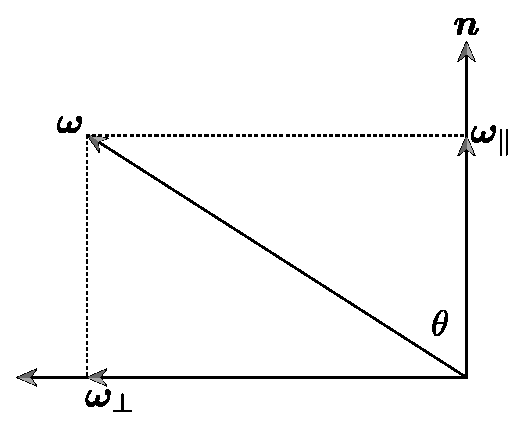
\includegraphics[width=0.4\linewidth]{Pictures/chap08/Parallelprojectionomeganormal.eps}
    \caption{向量$\bm\omega$在法线$\bm n$上的平行投影由${\bm\omega}_{\parallel}=(\cos\theta){\bm n}=({\bm n}\cdot{\bm\omega}){\bm n}$给出。
    垂直分量由${\bm\omega}_{\perp}=(\sin\theta){\bm n}$给出但用${\bm\omega}_{\perp}={\bm\omega}-{\bm\omega}_{\parallel}$计算更简单。}
    \label{fig:8.7}
\end{figure}

\reffig{8.8}展示了计算反射方向${\bm\omega}_{\mathrm{r}}$的设置。
我们可以看到两个向量都有相同的${\bm\omega}_{\parallel}$分量,
且${\bm\omega}_{\mathrm{r}\perp}$的值是${\bm\omega}_{\mathrm{o}\perp}$取反。
因此,我们有
\begin{align}
    \label{eq:8.5}
    {\bm\omega}_{\mathrm{r}}={\bm\omega}_{\mathrm{r}\perp}+{\bm\omega}_{\mathrm{r}\parallel} & =-{\bm\omega}_{\mathrm{o}\perp}+{\bm\omega}_{\mathrm{o}\parallel}\nonumber                                                        \\
                                                                                             & =-({\bm\omega}_{\mathrm{o}}-({\bm n}\cdot{\bm\omega}_{\mathrm{o}}){\bm n})+({\bm n}\cdot{\bm\omega}_{\mathrm{o}}){\bm n}\nonumber \\
                                                                                             & =-{\bm\omega}_{\mathrm{o}}+2({\bm n}\cdot{\bm\omega}_{\mathrm{o}}){\bm n}\, .
\end{align}
\begin{figure}[htbp]
    \centering
    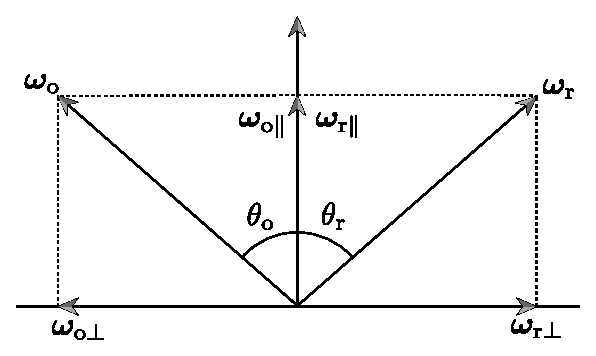
\includegraphics[width=0.5\linewidth]{Pictures/chap08/Perfectreflectioncomponents.eps}
    \caption{因为角$\theta_{\mathrm{o}}$和$\theta_{\mathrm{r}}$相等,
    所以完美反射方向的平行分量${\bm\omega}_{\mathrm{r}\parallel}$和
    入射方向的相同:${\bm\omega}_{\mathrm{r}\parallel}={\bm\omega}_{\mathrm{o}\parallel}$.
    其垂直分量就是入射方向垂直分量取反。}
    \label{fig:8.8}
\end{figure}

函数\refvar{Reflect}{()}实现了该计算。
\begin{lstlisting}
`\refcode{BSDF Inline Functions}{+=}\lastnext{BSDFInlineFunctions}`
inline `\refvar{Vector3f}{}` `\initvar{Reflect}{}`(const `\refvar{Vector3f}{}` &wo, const `\refvar{Vector3f}{}` &n) {
    return -wo + 2 * `\refvar{Dot}{}`(wo, n) * n;
}
\end{lstlisting}

在BRDF坐标系中,${\bm n}=(0,0,1)$,该表达式可极大简化。
\begin{lstlisting}
`\initcode{Compute perfect specular reflection direction}{=}`
*wi = `\refvar{Vector3f}{}`(-wo.x, -wo.y, wo.z);
\end{lstlisting}

\subsection{镜面透射}\label{sub:镜面透射}
\begin{lstlisting}
`\refcode{BSDF Inline Functions}{+=}\lastnext{BSDFInlineFunctions}`
inline bool `\initvar{Refract}{}`(const `\refvar{Vector3f}{}` &wi, const `\refvar{Normal3f}{}` &n, `\refvar{Float}{}` eta,
        `\refvar{Vector3f}{}` *wt) {
    `\refcode{Compute cos $\theta_t$ using Snell's law}{}`
    *wt = eta * -wi + (eta * cosThetaI - cosThetaT) * `\refvar{Vector3f}{}`(n);
    return true;
}
\end{lstlisting}

\section{朗伯反射}\label{sec:朗伯反射}

\section{微面模型}\label{sec:微面模型}

许多建模表面反射和透射的基于几何光学的方法
都基于一个观点即粗糙表面可以建模为
小的\keyindex{微面}{microfacet}{}合集。
由微面构成的曲面经常建模为高度场\sidenote{译者注:原文heightfield。},
其中微面的朝向分布是作统计上的描述。
\reffig{8.12}展示了相对粗糙表面的横截面和光滑得多的微面表面。
当区别不明显时,我们将用术语\keyindex{微曲面}{microsurface}{}来
描述微面曲面,用\keyindex{宏曲面}{macrosurface}{}来描述基本的光滑曲面
(即由\refvar{Shape}{}表示的)。
\begin{figure}[htbp]
    \centering
    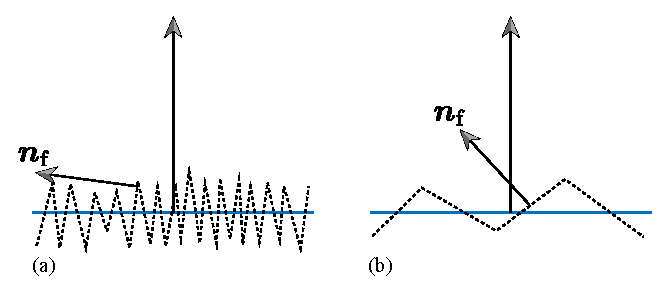
\includegraphics[width=0.75\linewidth]{Pictures/chap08/Roughsmoothmicrofacets.eps}
    \caption{微面曲面模型经常由给出微面法线${\bm n}_{\mathrm{f}}$关于
        曲面法线$\bm n$的分布的函数来描述。(a)微面法线变化越大,表面越粗糙。
        (b)光滑表面的微面法线变化相对较小。}
    \label{fig:8.12}
\end{figure}

基于微面的BRDF模型通过统计上对来自大量微面的光的散射建模来奏效。
如果我们假设被照明的微分区域$\mathrm{d}A$比起单个微面的尺寸相对大些,
则有大量微面被照亮且它们合起来的表现决定了观察到的散射。

微面模型的两个主要构成是\keyindex{刻面}{facet}{}
\sidenote{译者注:暂未查到facet在图形学中的专门翻译。}分布的表示
和描述光如何从单个微面散射的BRDF。有了这些,
任务是推导BRDF的解析表达式以描述来自这类曲面的散射。
尽管镜面透射对于建模许多透明材料很有用,
但对于微面BRDF,完美镜面反射是最常用的,
(下节介绍的)Oren-Nayar模型把微面看作朗伯反射体。

为了计算来自这类模型的反射,需要考虑微面级的局部光效应(\reffig{8.13})。
微面可能被另一刻面遮挡,可能处在相邻微面的阴影下,
或者\keyindex{互反射}{interreflection}{}可能
造成微面反射出比直接照明量和低层级微面BRDF预计的还多的光。
基于微面的特定BRDF模型以各种精确程度考虑了这些效应的每一种。
一般方法是做出尽可能最好的近似,且仍得到计算简单的表达式。
\begin{figure}[htbp]
    \centering
    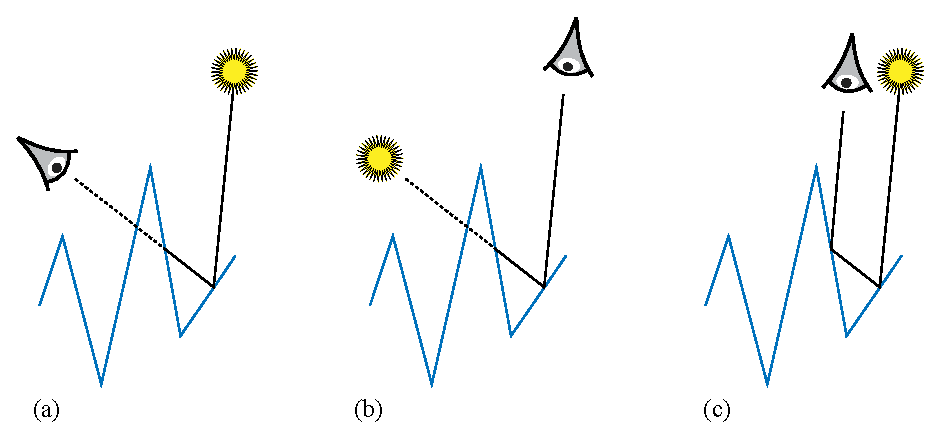
\includegraphics[width=\linewidth]{Pictures/chap08/Maskingshadowinginterreflection.eps}
    \caption{微面反射模型要考虑的三种重要几何效应。(a)遮掩(masking):
        考虑的微面因为另一微面的遮挡而对观察者不可见。(b)阴影(shadowing):
        类似地,光无法到达微面。(3)互反射:光在到达
        观察者之前于微面之间反弹。}
    \label{fig:8.13}
\end{figure}

\subsection{Oren-Nayar漫反射}\label{sub:Oren-Nayar漫反射}
\citet{10.1145/192161.192213}观察到真实世界物体不会展现完美朗伯反射。
具体地,当照明方向接近观察方向时,粗糙曲面通常显得更亮。
他们用含有单个参数$\sigma$即微面朝向角度标准差的球面高斯分布
描述的V形微面构建了描述粗糙曲面的反射模型。

在V形假设下,可以通过只考虑相邻微面来处理互反射;
\citeauthor{10.1145/192161.192213}利用这点
推导出对凹槽\sidenote{译者注:原文groove。}集的整体反射建模的BRDF。

所得模型考虑了微面间的阴影、遮掩和互反射,但没有解析解,
所以他们发现下列近似拟合得很好:
\begin{align*}
    f_{\mathrm{r}}({\bm\omega}_{\mathrm{i}},{\bm\omega}_{\mathrm{o}})=\frac{R}{\pi}(A+B\max(0,\cos(\varphi_{\mathrm{i}}-\varphi_{\mathrm{o}}))\sin\alpha\tan\beta)\, ,
\end{align*}
其中如果$\sigma$单位是弧度,则
\begin{align*}
    A      & =1-\frac{\sigma^2}{2(\sigma^2+0.33)}\, ,           \\
    B      & =\frac{0.45\sigma^2}{\sigma^2+0.09}\, ,            \\
    \alpha & =\max(\theta_{\mathrm{i}},\theta_{\mathrm{o}})\, , \\
    \beta  & =\min(\theta_{\mathrm{i}},\theta_{\mathrm{o}})\, .
\end{align*}

\begin{figure}[htbp]
    \centering
    \subfloat[朗伯]{\includegraphics[width=0.7\linewidth]{Pictures/chap08/f8-14a.png}\label{fig:8.14.1}}\\
    \subfloat[Oren-Nayar]{\includegraphics[width=0.7\linewidth]{Pictures/chap08/f8-14b.png}\label{fig:8.14.2}}
    \caption{(a)来自\refvar{LambertianReflection}{}模型的标准漫反射和
        (b)$\sigma$参数为20度的\refvar{OrenNayar}{}模型渲染的龙模型。
        注意用Oren-Nayar模型时暗色轮廓边缘反射增加了,浅色明暗边缘通常也更干脆
        (感谢Christian Schüller提供的模型)。}
    \label{fig:8.14}
\end{figure}

这里的实现在构造函数中预先计算和保存参数$A$与$B$的值
以节约稍后计算BRDF的工作量。\reffig{8.14}比较了理想漫反射和Oren-Nayar模型渲染的区别。
\begin{lstlisting}
`\initcode{OrenNayar Public Methods}{=}`
`\initvar{OrenNayar}{}`(const `\refvar{Spectrum}{}` &R, `\refvar{Float}{}` sigma) 
    : `\refvar{BxDF}{}`(`\refvar{BxDFType}{}`(`\refvar[BSDFREFLECTION]{BSDF\_REFLECTION}{}` | `\refvar[BSDFDIFFUSE]{BSDF\_DIFFUSE}{}`)), `\refvar[OrenNayar::R]{R}{}`(R) {
    sigma = `\refvar{Radians}{}`(sigma);
    `\refvar{Float}{}` sigma2 = sigma * sigma;
    `\refvar[OrenNayar::A]{A}{}` = 1.f - (sigma2 / (2.f * (sigma2 + 0.33f)));
    `\refvar[OrenNayar::B]{B}{}` = 0.45f * sigma2 / (sigma2 + 0.09f);
}
\end{lstlisting}
\begin{lstlisting}
`\initcode{OrenNayar Private Data}{=}`
const `\refvar{Spectrum}{}` `\initvar[OrenNayar::R]{R}{}`;
`\refvar{Float}{}` `\initvar[OrenNayar::A]{A}{}`, `\initvar[OrenNayar::B]{B}{}`;
\end{lstlisting}

比起直接变换基本方程,三角恒等式的应用可以极大提升求值例程的效率。
实现从计算$\sin\theta_{\mathrm{i}}$和$\sin\theta_{\mathrm{o}}$的值开始。
\begin{lstlisting}
`\refcode{BxDF Method Definitions}{+=}\lastnext{BxDFMethodDefinitions}`
`\refvar{Spectrum}{}` `\refvar{OrenNayar}{}`::`\initvar[OrenNayar::f]{f}{}`(const `\refvar{Vector3f}{}` &wo, const `\refvar{Vector3f}{}` &wi) const {
    `\refvar{Float}{}` sinThetaI = `\refvar{SinTheta}{}`(wi);
    `\refvar{Float}{}` sinThetaO = `\refvar{SinTheta}{}`(wo);
    `\refcode{Compute cosine term of Oren-Nayar model}{}`
    `\refcode{Compute sine and tangent terms of Oren-Nayar model}{}`
    return `\refvar[OrenNayar::R]{R}{}` * `\refvar{InvPi}{}` * (`\refvar[OrenNayar::A]{A}{}` + `\refvar[OrenNayar::B]{B}{}` * maxCos * sinAlpha * tanBeta);
}
\end{lstlisting}

为了计算项$\max(0,\cos(\varphi_{\mathrm{i}}-\varphi_{\mathrm{o}}))$,
我们可以应用三角恒等式
\begin{align*}
    \cos(a-b)=\cos a\cos b+\sin a\sin b\, ,
\end{align*}
这样我们只需要计算$\varphi_{\mathrm{i}}$和$\varphi_{\mathrm{o}}$的正弦和余弦。
\begin{lstlisting}
`\initcode{Compute cosine term of Oren-Nayar model}{=}`
`\refvar{Float}{}` maxCos = 0;
if (sinThetaI > 1e-4 && sinThetaO > 1e-4) {
    `\refvar{Float}{}` sinPhiI = `\refvar{SinPhi}{}`(wi), cosPhiI = `\refvar{CosPhi}{}`(wi);
    `\refvar{Float}{}` sinPhiO = `\refvar{SinPhi}{}`(wo), cosPhiO = `\refvar{CosPhi}{}`(wo);
    `\refvar{Float}{}` dCos = cosPhiI * cosPhiO + sinPhiI * sinPhiO;
    maxCos = std::max((`\refvar{Float}{}`)0, dCos);
}
\end{lstlisting}

最后,求得项$\sin\alpha$和$\tan\beta$.
注意无论${\bm\omega}_{\mathrm{i}}$或${\bm\omega}_{\mathrm{o}}$中的哪一个,
有更大的$\cos\theta$(即更大的$z$分量)就有更小的$\theta$.
我们可以用该方法开头计算的近似正弦值来设定$\sin\alpha$.
然后用恒等式$\displaystyle\tan\theta=\frac{\sin\theta}{\cos\theta}$计算正切。
\begin{lstlisting}
`\initcode{Compute sine and tangent terms of Oren-Nayar model}{=}`
`\refvar{Float}{}` sinAlpha, tanBeta;
if (`\refvar{AbsCosTheta}{}`(wi) > `\refvar{AbsCosTheta}{}`(wo)) {
    sinAlpha = sinThetaO;
    tanBeta = sinThetaI / `\refvar{AbsCosTheta}{}`(wi);
} else {
    sinAlpha = sinThetaI;
    tanBeta = sinThetaO / `\refvar{AbsCosTheta}{}`(wo);
}
\end{lstlisting}

\subsection{微面分布函数}\label{sub:微面分布函数}
反射模型所基于的微面展现出完美镜面反射和透射时,
其对来自各种光泽材料的光散射的建模已经很高效了,包括金属、塑料和磨砂玻璃。
在我们讨论这些模型的辐射度量细节前,
我们将首先介绍概括了其几何属性的抽象。
这里的代码包括了两个广泛使用的微面模型的实现。
这些代码都在文件\href{https://github.com/mmp/pbrt-v3/tree/master/src/core/microfacet.h}{\ttfamily core/microfacet.h}
和\href{https://github.com/mmp/pbrt-v3/tree/master/src/core/microfacet.cpp}{\ttfamily core/microfacet.cpp}中。

\refvar{MicrofacetDistribution}{}定义了
由微面实现提供的接口及其常用功能。
\begin{lstlisting}
`\initcode{MicrofacetDistribution Declarations}{=}\initnext{MicrofacetDistributionDeclarations}`
class `\initvar{MicrofacetDistribution}{}` {
public:
    `\refcode{MicrofacetDistribution Public Methods}{}`
protected:
    `\refcode{MicrofacetDistribution Protected Methods}{}`
    `\refcode{MicrofacetDistribution Protected Data}{}`
};
\end{lstlisting}

微面曲面的一个重要特性由分布函数$D({\bm\omega}_{\mathrm{h}})$表示,
它给出了曲面法线为${\bm\omega}_{\mathrm{h}}$的微面的微分面积
(回想\reffig{8.12}展示了曲面的粗糙度是怎样和微面法线分布函数相联系的)。
在pbrt中,微面分布函数和\refvar{BxDF}{}在相同的BSDF坐标系下定义;
这样,完全光滑的曲面可由仅当${\bm\omega}_{\mathrm{h}}$等于
曲面法线时才取非零值的$\delta$分布描述:$D({\bm\omega}_{\mathrm{h}})=\delta({\bm\omega}_{\mathrm{h}}-(0,0,1))$.

微面分布函数必须规范化以保证它们的物理合理性
\sidenote{译者注:除了下文的归一化约束,$D({\bm\omega}_{\mathrm{h}})$还有非负性。}。
直观上,如果我们考虑微曲面上沿法线方向$\bm n$的入射光线,
则每条光线一定和微面曲面恰好相交一次。更形式化地,
给定微曲面的微分面积$\mathrm{d}A$,则该区域之上微面的投影面积
一定等于$\mathrm{d}A$(\reffig{8.15})
\sidenote{译者注:该公式积分区域取半空间并不严谨,实际上应取全空间才对,否则会漏掉背面朝向的微面面积。
    有关$D({\bm\omega}_{\mathrm{h}})$的详细说明可参见笔者编写的\refsec{译者补充:微面模型相关推导}。}。
数学上,这对应着以下条件
\footnote{规范化微面分布的常见错误是在整个立体角上
    而不是投影立体角上执行该积分(即略去的项$\cos\theta_{\mathrm{h}}$),
    这无法保证具有正确分布的高度场存在。}:
\begin{align*}
    \int\limits_{H^2({\bm n})}D({\bm\omega}_{\mathrm{h}})\cos\theta_{\mathrm{h}}\mathrm{d}{\bm\omega}_{\mathrm{h}}=1\, .
\end{align*}
\begin{figure}[htbp]
    \centering
    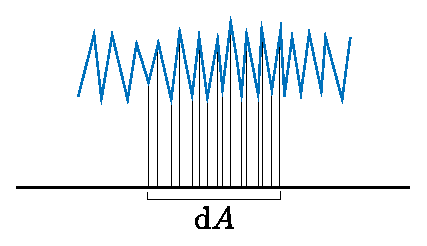
\includegraphics[width=0.5\linewidth]{Pictures/chap08/MicrofacetnormalizedA.eps}
    \caption{给定曲面上的微分面积$\mathrm{d}A$,
        则微面法线分布函数$D({\bm\omega}_{\mathrm{h}})$必须规范化使得
        该区域上的微面的投影曲面面积等于$\mathrm{d}A$.}
    \label{fig:8.15}
\end{figure}

方法\refvar{MicrofacetDistribution::D}{()}对应函数$D({\bm\omega}_{\mathrm{h}})$;
实现返回具有给定法线向量$\omega$朝向的微面的微分面积。
\begin{lstlisting}
`\initcode{MicrofacetDistribution Public Methods}{=}\initnext{MicrofacetDistributionPublicMethods}`
virtual `\refvar{Float}{}` `\initvar[MicrofacetDistribution::D]{D}{}`(const `\refvar{Vector3f}{}` &wh) const = 0;
\end{lstlisting}

\citet{1987BeckmannSpizzichino}\sidenote{译者注:
    笔者只查到了1987年同名同作者书籍,原文引用为1963年。}提出了
一种广泛使用的基于微面斜率高斯分布的微面分布函数;
我们的实现在类\refvar{BeckmannDistribution}{}中。
\begin{lstlisting}
`\refcode{MicrofacetDistribution Declarations}{+=}\lastnext{MicrofacetDistributionDeclarations}`
class `\initvar{BeckmannDistribution}{}` : public `\refvar{MicrofacetDistribution}{}` {
public:
    `\refcode{BeckmannDistribution Public Methods}{}`
private:
    `\refcode{BeckmannDistribution Private Methods}{}`
    `\refcode{BeckmannDistribution Private Data}{}`
};
\end{lstlisting}

Beckmann-Spizzichino模型的传统定义是
\begin{align}\label{eq:8.9}
    D({\bm\omega}_{\mathrm{h}})=\frac{\mathrm{e}^{-\frac{\tan^2\theta_{\mathrm{h}}}{\alpha^2}}}{\pi\alpha^2\cos^4\theta_{\mathrm{h}}}\, ,
\end{align}
其中如果$\sigma$是微面斜率的均方根\sidenote{译者注:原文RMS。},则$\alpha=\sqrt{2}\sigma$.

定义各向异性分布很有用,即法线分布也随${\bm\omega}_{\mathrm{h}}$的
方位朝向变化。例如,所朝方向垂直于$x$轴的微面对应记为$\alpha_x$,
而$y$轴的为$\alpha_y$,则中间朝向的$\alpha$值可用通过这些值构造的椭圆来插值。

对应的各向异性微面分布函数为
\sidenote{译者注:\refsec{译者补充:微面模型相关推导},
    给出了本节微面分布模型满足规范性的证明。}
\begin{align}\label{eq:8.10}
    D({\bm\omega}_{\mathrm{h}})=\frac{\mathrm{e}^{-\left(\frac{\cos^2\varphi_{\mathrm{h}}}{\alpha_x^2}+\frac{\sin^2\varphi_{\mathrm{h}}}{\alpha_y^2}\right)\tan^2\theta_{\mathrm{h}}}}{\pi\alpha_x\alpha_y\cos^4\theta_{\mathrm{h}}}\, .
\end{align}
注意当$\alpha_x=\alpha_y$时Beckmann-Spizzichino模型
变为原始的各向同性版本。

成员变量\refvar[BeckmannDistribution::alphax]{alphax}{}和
\refvar[BeckmannDistribution::alphay]{alphay}{}都在
\refvar{BeckmannDistribution}{}的构造函数中设定,
它很简单所以这里不再介绍。
\begin{lstlisting}
`\initcode{BeckmannDistribution Private Data}{=}`
const `\refvar{Float}{}` `\initvar[BeckmannDistribution::alphax]{alphax}{}`, `\initvar[BeckmannDistribution::alphay]{alphay}{}`;
\end{lstlisting}

方法\refvar{BeckmannDistribution::D}{()}直接翻译了\refeq{8.10}。
仅有的额外实现细节是必须特殊处理$\tan^2\theta$的无限值。
该情况实际上是有效的——它在完全扫掠的方向上发生。
该情况下,下面的代码最终企图计算$\displaystyle\frac{0}{0}$,
这会得到“not a number”(NaN)值,最终导致为当前像素样本的辐射亮度返回NaN值。
因此,为该情况明确地返回零,也即当$\tan^2\theta_{\mathrm{h}}$趋向
无穷大时$D({\bm\omega}_{\mathrm{h}})$收敛的值。
\begin{lstlisting}
`\initcode{MicrofacetDistribution Method Definitions}{=}\initnext{MicrofacetDistributionMethodDefinitions}`
`\refvar{Float}{}` `\refvar{BeckmannDistribution}{}`::`\initvar[BeckmannDistribution::D]{D}{}`(const `\refvar{Vector3f}{}` &wh) const {
    `\refvar{Float}{}` tan2Theta = `\refvar{Tan2Theta}{}`(wh);
    if (std::isinf(tan2Theta)) return 0.;
    `\refvar{Float}{}` cos4Theta = `\refvar{Cos2Theta}{}`(wh) * `\refvar{Cos2Theta}{}`(wh);
    return std::exp(-tan2Theta * (`\refvar{Cos2Phi}{}`(wh) / (`\refvar[BeckmannDistribution::alphax]{alphax}{}` * `\refvar[BeckmannDistribution::alphax]{alphax}{}`) +
                                  `\refvar{Sin2Phi}{}`(wh) / (`\refvar[BeckmannDistribution::alphay]{alphay}{}` * `\refvar[BeckmannDistribution::alphay]{alphay}{}`))) /
        (`\refvar{Pi}{}` * `\refvar[BeckmannDistribution::alphax]{alphax}{}` * `\refvar[BeckmannDistribution::alphay]{alphay}{}` * cos4Theta);
}
\end{lstlisting}

\citet{Trowbridge:75}提出了另一个有用的微面分布函数
\footnote{该模型也由\citet{10.5555/2383847.2383874}独立推导出,称作“GGX”。}。
其各向异性变体由下式给出:
\begin{align}\label{eq:8.11}
    D({\bm\omega}_{\mathrm{h}})=\frac{1}{\pi\alpha_x\alpha_y\left(1+\left(\frac{\cos^2\varphi_{\mathrm{h}}}{\alpha_x^2}+\frac{\sin^2\varphi_{\mathrm{h}}}{\alpha_y^2}\right)\tan^2\theta_{\mathrm{h}}\right)^2\cos^4\theta_{\mathrm{h}}}\, .
\end{align}

相比于Beckmann-Spizzichino模型,Trowbridge-Reitz模型有更高的拖尾——
在远离曲面法线的方向上它会更慢地降到零。该特性与许多真实世界表面的性质吻合得很好。
见\reffig{8.16}中这两个微面分布函数的图示。
\begin{figure}[htbp]
    \centering
    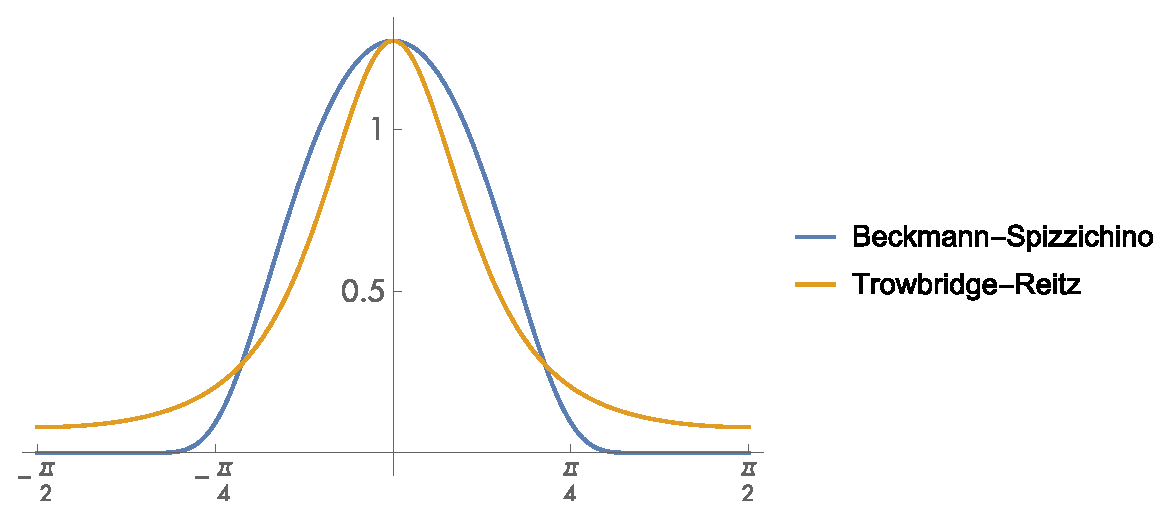
\includegraphics[width=0.75\linewidth]{Pictures/chap08/beckmann-vs-tr-tails.eps}
    \caption{当$\alpha=0.5$时各向同性的Beckmann-Spizzichino和Trowbridge-Reitz微面分布函数
        关于$\theta$的函数图像。注意Trowbridge-Reitz对于更大量级的$\theta$有更高的尾部。}
    \label{fig:8.16}
\end{figure}

\begin{lstlisting}
`\refcode{MicrofacetDistribution Declarations}{+=}\lastnext{MicrofacetDistributionDeclarations}`
class `\initvar{TrowbridgeReitzDistribution}{}` : public `\refvar{MicrofacetDistribution}{}` {
public:
    `\refcode{TrowbridgeReitzDistribution Public Methods}{}`
private:
    `\refcode{TrowbridgeReitzDistribution Private Methods}{}`
    `\refcode{TrowbridgeReitzDistribution Private Data}{}`
};
\end{lstlisting}

比起直接指定$\alpha$的值,用一个$[0,1]$中的标量参数来
指定BRDF的粗糙度会很方便,其中接近零的值对应几乎完美的镜面反射。
这里略去的方法\refvar{RoughnessToAlpha}{()}执行从该粗糙度值到$\alpha$值的映射。
\begin{lstlisting}
`\initcode{TrowbridgeReitzDistribution Public Methods}{=}`
static inline `\refvar{Float}{}` `\initvar{RoughnessToAlpha}{}`(`\refvar{Float}{}` roughness);
\end{lstlisting}
\begin{lstlisting}
`\initcode{TrowbridgeReitzDistribution Private Data}{=}`
const `\refvar{Float}{}` `\initvar[TrowbridgeReitzDistribution::alphax]{alphax}{}`, `\initvar[TrowbridgeReitzDistribution::alphay]{alphay}{}`;
\end{lstlisting}

方法\refvar[TrowbridgeReitzDistribution::D]{D}{()}是直接照着\refeq{8.11}写的。
\begin{lstlisting}
`\refcode{MicrofacetDistribution Method Definitions}{+=}\lastnext{MicrofacetDistributionMethodDefinitions}`
`\refvar{Float}{}` `\refvar{TrowbridgeReitzDistribution}{}`::`\initvar[TrowbridgeReitzDistribution::D]{D}{}`(const `\refvar{Vector3f}{}` &wh) const {
    `\refvar{Float}{}` tan2Theta = `\refvar{Tan2Theta}{}`(wh);
    if (std::isinf(tan2Theta)) return 0.;
    const `\refvar{Float}{}` cos4Theta = `\refvar{Cos2Theta}{}`(wh) * `\refvar{Cos2Theta}{}`(wh);
    `\refvar{Float}{}` e = (`\refvar{Cos2Phi}{}`(wh) / (`\refvar[TrowbridgeReitzDistribution::alphax]{alphax}{}` * `\refvar[TrowbridgeReitzDistribution::alphax]{alphax}{}`) +
               `\refvar{Sin2Phi}{}`(wh) / (`\refvar[TrowbridgeReitzDistribution::alphay]{alphay}{}` * `\refvar[TrowbridgeReitzDistribution::alphay]{alphay}{}`)) * tan2Theta;
    return 1 / (`\refvar{Pi}{}` * `\refvar[TrowbridgeReitzDistribution::alphax]{alphax}{}` * `\refvar[TrowbridgeReitzDistribution::alphay]{alphay}{}` * cos4Theta * (1 + e) * (1 + e));
}
\end{lstlisting}

\subsection{掩模和遮挡}\label{sub:掩模和遮挡}
对于渲染,只有微面法线分布不足以完全表征微曲面。
同样很重要的是,要考虑到一些微面从某给定视角或光照方向看去
会因为它们是背面朝向而不可见(因而其他微面在它们的前方),
以及一些正面朝向的微面区域会因为受到背面朝向微面的遮挡而被隐藏。
Smith的\keyindex{掩模遮挡函数}{masking-shadowing function}{}
$G_1({\bm\omega},{\bm\omega}_{\mathrm{h}})$考虑了这些效应,
给出了从方向$\bm\omega$可见且法线为${\bm\omega}_{\mathrm{h}}$的微面比例
(注意$0\le G_1({\bm\omega},{\bm\omega}_{\mathrm{h}})\le 1$)。
通常情况下微面可见的概率独立于其朝向${\bm\omega}_{\mathrm{h}}$,
我们可以把该函数写作$G_1({\bm\omega})$.

如\reffig{8.17}所示,从和曲面法线夹角为$\theta$的方向$\bm\omega$上
去观察曲面上的微分面积$\mathrm{d}A$时看到的面积为$\mathrm{d}A\cos\theta$.
从该方向可见的微面面积也一定等于$\mathrm{d}A\cos\theta$,
由此导出对$G_1$的规范化约束:
\begin{align}
    \label{eq:8.12}
    \cos\theta=\int\limits_{H^2({\bm n})}G_1({\bm\omega},{\bm\omega}_{\mathrm{h}})\max(0,{\bm\omega}\cdot{\bm\omega}_{\mathrm{h}})D({\bm\omega}_{\mathrm{h}})\mathrm{d}{\bm\omega}_{\mathrm{h}}\, .
\end{align}
换句话说,对给定方向$\bm\omega$可见的微面的投影面积一定等于
宏曲面微分面积$\mathrm{d}A$的$({\bm\omega}\cdot{\bm n})=\cos\theta$倍。

\begin{figure}[htbp]
    \centering
    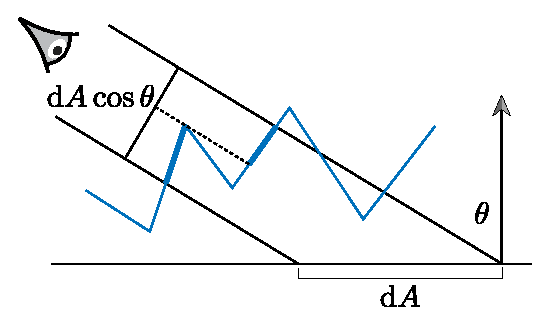
\includegraphics[width=0.5\linewidth]{Pictures/chap08/Microfacetvisiblearea.eps}
    \caption{从观察者或光源处看时,曲面上的微分面积变为$\mathrm{d}A\cos\theta$,
        其中$\cos\theta$是入射方向与曲面法线夹角的余弦。
        可见微面(粗线)的投影曲面面积也一定等于$\mathrm{d}A\cos\theta$;
        掩模遮挡函数$G_1$给出了$\mathrm{d}A$上的微面总面积中在给定方向可见的比例。}
    \label{fig:8.17}
\end{figure}

因为微面构成了高度场,所以每个背向微面遮住的正向微面面积
都等于它在方向$\bm\omega$的投影面积。
\refeq{8.12}中,如果$A^{+}({\bm\omega})$是从方向$\bm\omega$看到的
正向微面投影面积,而$A^{-}({\bm\omega})$是背向微面的投影面积,
则$\cos\theta=A^{+}({\bm\omega})-A^{-}({\bm\omega})$.
因此我们可以把掩模遮挡函数改写为可见微面面积与正向微面面积之比:
\begin{align*}
    G_1({\bm\omega})=\frac{A^{+}({\bm\omega})-A^{-}({\bm\omega})}{A^{+}({\bm\omega})}\, .
\end{align*}

掩模遮挡函数习惯上用一个辅助函数$\Lambda({\bm\omega})$来表示,
后者度量了单位可见微面面积内被遮挡不可见的微面面积。
\begin{align}
    \label{eq:8.13}
    \Lambda({\bm\omega})=\frac{A^{-}({\bm\omega})}{A^{+}({\bm\omega})-A^{-}({\bm\omega})}=\frac{A^{-}({\bm\omega})}{\cos\theta}\, .
\end{align}

方法\refvar[MicrofacetDistribution::Lambda]{Lambda}{()}计算该函数。对于每个微面分布它都有特定实现。
\begin{lstlisting}
`\refcode{MicrofacetDistribution Public Methods}{+=}\lastnext{MicrofacetDistributionPublicMethods}`
virtual `\refvar{Float}{}` `\initvar[MicrofacetDistribution::Lambda]{Lambda}{}`(const `\refvar{Vector3f}{}` &w) const = 0;
\end{lstlisting}

我们通过一些代数变换用$\Lambda({\bm\omega})$表示$G_1({\bm\omega})$:
\begin{align*}
    G_1({\bm\omega})=\frac{1}{1+\Lambda({\bm\omega})}\, ,
\end{align*}
因此我们利用\refvar[MicrofacetDistribution::Lambda]{Lambda}{()}来
提供方法\refvar[MicrofacetDistribution::G1]{G1}{()}。
\begin{lstlisting}
`\refcode{MicrofacetDistribution Public Methods}{+=}\lastnext{MicrofacetDistributionPublicMethods}`
`\refvar{Float}{}` `\initvar[MicrofacetDistribution::G1]{G1}{}`(const `\refvar{Vector3f}{}` &w) const {
    return 1 / (1 + `\refvar[MicrofacetDistribution::Lambda]{Lambda}{}`(w));
}
\end{lstlisting}

只是微面分布还不能施加足够的条件以明确一个特定的$\Lambda({\bm\omega})$函数;
许多函数都能满足\refeq{8.12}中的约束。
例如,如果我们假设微面上邻近点的高度之间没有关联,
则可能为给定的$D({\bm\omega}_{\mathrm{h}})$找到唯一的$\Lambda({\bm\omega})$
(对于许多微面模型来说都能找到解析解)。
尽管该基本假设在现实中不成立——对于实际的微面,
一点的高度通常接近邻近点的高度——但所得函数$\Lambda({\bm\omega})$与
从实际表面测量到的情况相比已经很精确了。

在邻近点高度无关的假设下,各向同性的Beckmann-Spizzichino分布的$\Lambda({\bm\omega})$是
\begin{align}
    \Lambda({\bm\omega})=\frac{1}{2}\left(\mathrm{erf}(a)-1+\frac{\mathrm{e}^{-a^2}}{a\sqrt{\pi}}\right)\, ,
\end{align}
其中$a=\displaystyle\frac{1}{\alpha\tan\theta}$,而$\mathrm{erf}$是
误差函数,$\displaystyle\mathrm{erf}(x)=\frac{2}{\sqrt{\pi}}\int_0^x\mathrm{e}^{-x'^2}\mathrm{d}x'$.


\section{菲涅耳入射效应}\label{sec:菲涅耳入射效应}
图形学中许多BRDF模型都没有考虑到菲涅耳反射会减少到达多层物体底层光量的事实。
考虑一张抛光的木桌或者涂了光泽油漆的墙面:如果你正对着看向它们的表面,
你主要看到的是木头或油漆颜料的颜色。随着你把你的视角移向掠角,
你会看到更少的底色,因为它被随菲涅耳效应而增加的光泽反射淹没了。

本节中,我们将实现由\citet{AshikhminPhong,Ashikhmin01012000}
\sidenote{译者注:原文文献年份标注可能有误,已修正。}
开发的BRDF模型,它刻画了覆盖有光泽镜面表面的漫反射表面。
在考虑了菲涅耳效应后,来自漫反射曲面的的反射效应会由剩余能量量值调制。
\reffig{8.23}展示了该想法:当入射方向接近法线时,大部分光会透射到
漫反射层,漫反射项占主要部分。而当入射方向接近掠角时,主要反射模式则是光泽反射。
\reffig{12.19}的汽车模型就给它的车漆用的本模型。
\begin{lstlisting}
`\refcode{BxDF Declarations}{+=}\lastnext{BxDFDeclarations}`
class `\initvar{FresnelBlend}{}` : public `\refvar{BxDF}{}` {
public:
    `\refcode{FresnelBlend Public Methods}{}`
private:
    `\refcode{FresnelBlend Private Data}{}`
};
\end{lstlisting}

\begin{figure}[htbp]
    \centering
    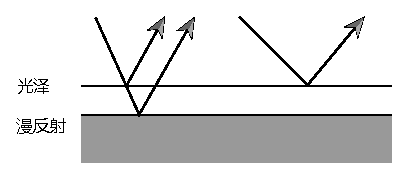
\includegraphics[width=0.65\linewidth]{Pictures/chap08/Fresnelincidence.eps}
    \caption{\refvar{FresnelBlend}{} BRDF刻画漫反射底层之上具有光泽层的曲面效果。
    随着向量${\bm\omega}_{\mathrm{i}}$和${\bm\omega}_{\mathrm{o}}$射入的角度移向掠角(右例),
    到达漫反射底层的光量因菲涅耳效应而减少,漫反射层变得更不明显了。}
    \label{fig:8.23}
\end{figure}

该模型接收两个光谱,一个表示漫反射和镜面反射,一个为光泽层的微面分布。
\begin{lstlisting}
`\refcode{BxDF Method Definitions}{+=}\lastnext{BxDFMethodDefinitions}`
`\refvar{FresnelBlend}{}`::`\refvar{FresnelBlend}{}`(const `\refvar{Spectrum}{}` &Rd, const `\refvar{Spectrum}{}` &Rs,
                           `\refvar{MicrofacetDistribution}{}` *distribution) 
    : `\refvar{BxDF}{}`(`\refvar{BxDFType}{}`(`\refvar[BSDFREFLECTION]{BSDF\_REFLECTION}{}` | `\refvar[BSDFGLOSSY]{BSDF\_GLOSSY}{}`)),
      `\refvar[FresnelBlend::Rd]{Rd}{}`(Rd), `\refvar[FresnelBlend::Rs]{Rs}{}`(Rs), `\refvar[FresnelBlend::distribution]{distribution}{}`(distribution) { }
\end{lstlisting}
\begin{lstlisting}
`\initcode{FresnelBlend Private Data}{=}`
const `\refvar{Spectrum}{}` `\initvar[FresnelBlend::Rd]{Rd}{}`, `\initvar[FresnelBlend::Rs]{Rs}{}`;
`\refvar{MicrofacetDistribution}{}` *`\initvar[FresnelBlend::distribution]{distribution}{}`;
\end{lstlisting}

该模型基于光泽镜面项和漫反射项的加权和。考虑到互易性和能量守恒,推导出光泽镜面项为
\sidenote{译者注:原文漏写了$F_{\mathrm{r}}$的下标,已修正。}
\begin{align*}
    f_{\mathrm{r}}({\bm p},{\bm\omega}_{\mathrm{o}},{\bm\omega}_{\mathrm{i}})
    =\frac{D({\bm\omega}_{\mathrm{h}})F_{\mathrm{r}}({\bm\omega}_{\mathrm{o}})}
    {4({\bm\omega}_{\mathrm{h}}\cdot{\bm\omega}_{\mathrm{i}})
    (\max(({\bm n}\cdot{\bm\omega}_{\mathrm{o}}),({\bm n}\cdot{\bm\omega}_{\mathrm{i}})))}\, ,
\end{align*}
其中$D({\bm\omega}_{\mathrm{h}})$是微面分布项,$F_{\mathrm{r}}({\bm\omega}_{\mathrm{o}})$表示
菲涅耳反射率。注意它和Torrance-Sparrow模型非常像。
\citeauthor{AshikhminPhong}的模型的关键是推导出仍然遵循互易性和
能量守恒的漫反射项。其推导依赖于\citet{Schlick1993}给出的对菲涅耳反射方程的近似,即
\sidenote{译者注:原文以$\theta$来表示代入的角度变量,但可能引起歧义,
实际上该论文代入的角度是半角大小$\theta_{\mathrm{h}}$,译文已修改。}
\begin{align*}
    F_{\mathrm{r}}(\cos\theta_{\mathrm{h}})=R+(1-R)(1-\cos\theta_{\mathrm{h}})^5\, ,
\end{align*}
其中$R$是按法线入射时的曲面反射率。

有了该菲涅耳项,下式的漫反射项就能以物理上较合理的方式成功刻画基于菲涅耳衰减的漫反射。
\begin{align*}
    f_{\mathrm{r}}({\bm p},{\bm\omega}_{\mathrm{o}},{\bm\omega}_{\mathrm{i}})
    =\frac{28R_{\mathrm{d}}}{23\pi}(1-R_{\mathrm{s}})
    \left(1-\left(1-\frac{1}{2}({\bm n}\cdot{\bm\omega}_{\mathrm{i}})\right)^5\right)
    \left(1-\left(1-\frac{1}{2}({\bm n}\cdot{\bm\omega}_{\mathrm{o}})\right)^5\right)\, .
\end{align*}

我们不会在这里引入对该结果的推导。
\begin{lstlisting}
`\initcode{FresnelBlend Public Methods}{=}`
`\refvar{Spectrum}{}` `\initvar{SchlickFresnel}{}`(`\refvar{Float}{}` cosTheta) const {
    auto pow5 = [](`\refvar{Float}{}` v) { return (v * v) * (v * v) * v; };
    return `\refvar[FresnelBlend::Rs]{Rs}{}` + pow5(1 - cosTheta) * (`\refvar{Spectrum}{}`(1.) - `\refvar[FresnelBlend::Rs]{Rs}{}`);
}
\end{lstlisting}
\begin{lstlisting}
`\refcode{BxDF Method Definitions}{+=}\lastnext{BxDFMethodDefinitions}`
`\refvar{Spectrum}{}` `\refvar{FresnelBlend}{}`::`\initvar[FresnelBlend::f]{f}{}`(const `\refvar{Vector3f}{}` &wo, const `\refvar{Vector3f}{}` &wi) const {
    auto pow5 = [](`\refvar{Float}{}` v) { return (v * v) * (v * v) * v; };
    `\refvar{Spectrum}{}` diffuse = (28.f/(23.f*`\refvar{Pi}{}`)) * `\refvar[FresnelBlend::Rd]{Rd}{}` *
        (`\refvar{Spectrum}{}`(1.f) - `\refvar[FresnelBlend::Rs]{Rs}{}`) * 
        (1 - pow5(1 - .5f * `\refvar{AbsCosTheta}{}`(wi))) *
        (1 - pow5(1 - .5f * `\refvar{AbsCosTheta}{}`(wo)));
    `\refvar{Vector3f}{}` wh = wi + wo;
    if (wh.x == 0 && wh.y == 0 && wh.z == 0) return `\refvar{Spectrum}{}`(0);
    wh = `\refvar{Normalize}{}`(wh);
    `\refvar{Spectrum}{}` specular = `\refvar[FresnelBlend::distribution]{distribution}{}`->`\refvar[MicrofacetDistribution::D]{D}{}`(wh) /
        (4 * `\refvar{AbsDot}{}`(wi, wh) *
         std::max(`\refvar{AbsCosTheta}{}`(wi), `\refvar{AbsCosTheta}{}`(wo))) *
         `\refvar{SchlickFresnel}{}`(`\refvar{Dot}{}`(wi, wh));
    return diffuse + specular;
}
\end{lstlisting}


\section{傅里叶基BSDF}\label{sec:傅里叶基BSDF}
尽管像Torrance-Sparrow和Oren-Nayar这样的模型可以准确地表示许多材料,
但一些材料所拥有的BRDF形态并不能很好地匹配这些模型
(例如带有光滑或粗糙涂料或面料的金属等分层材料,它们通常是部分反光的)。
针对这类材料的一个办法是把它们的BSDF值存进一个
巨大的3D或4D\keyindex{查找表}{lookup table}{},
但是该方法需要难以接受的存储量——例如,
如果${\bm\omega}_{\mathrm{i}}$和${\bm\omega}_{\mathrm{o}}$都按1度间隔
在球面角内采样,则以4D查找表的形式表示相应各向异性BSDF需要超过十亿个样本点。

因此,我们很需要有一个更紧凑的方式来依然准确表示BSDF。
本节介绍的\refvar{FourierBSDF}{}利用傅里叶基,
以缩放的余弦项之和表示BSDF。该表示既准确又节约空间,并能与蒙特卡罗积分很好地配合
(见\refsub{傅里叶BSDF})。\reffig{8.24}展示了用这种表示渲染的两个龙模型的例子。
\begin{figure}[htbp]
    \centering
    \includegraphics[width=\linewidth]{Pictures/chap08/dragons-fourier.png}
    \caption{用\refvar{FourierBSDF}{}模型渲染的龙模型。
    左边龙表面的BSDF建模了粗糙黄金的外观;右边的则是镀铜(感谢Christian Schüller提供模型)。}
    \label{fig:8.24}
\end{figure}

这里我们不会讨论BSDF是如何转换成这种表示的,但我们会关注它在渲染中的应用。
详见本章末的“扩展阅读”一节了解这些问题的更多细节以及
pbrt发行中路径\href{https://pbrt.org/scenes-v3}{\ttfamily bsdfs}下各种以此格式表示的BSDF。


\section{扩展阅读}\label{sec:扩展阅读08}
\citet{10.1145/360825.360839}为计算机图形学中的光泽曲面开发了早期经验反射模型。
尽管它既不互易也不能量守恒,但它是非朗伯体的首张合成图像的基石。
\citet{Torrance:67}阐述了Torrance-Sparrow微面模型;
\citet{10.1145/965141.563893}首次将它引入图形学,
\citet{10.1145/800224.806819,10.1145/357290.357293}则使用了它的变体。
Oren-Nayar朗伯模型在他们\citeyear{10.1145/192161.192213}年
的论文\citep{10.1145/192161.192213}中得到阐述。

\citet{10.1007/978-1-4612-3526-2}的书籍总结并阐述了
当时图形学中最好的基于物理的曲面反射模型。
该书详细讨论了曲面反射的物理性质,并附有许多原文指引和
从真实曲面测得的关于反射的实用数据表格。
\citet{Burley:2012:PBS}最近的论文包含了计算机图形学
反射模型近期工作的详尽注解书目。

\citet{heitz:hal-01024289}关于微面掩模遮挡函数的论文
对微面BSDF模型的整体介绍写得非常好,并附有关于这一话题细节许多有用的图示和解释。
参见\citet{1987BeckmannSpizzichino}与\citet{Trowbridge:75}的
论文分别对他们的微面分布函数的介绍。
\citet{10.1145/1722991.1722996}开发了各向异性Beckmann-Spizzichino分布函数;
参见\citet{heitz:hal-01024289}了解其他许多微面分布函数的各向异性版本。
计算机图形学的早期各向异性BRDF模型由\citet{10.1145/325334.325167}、
\citet{10.1145/97879.97909}开发。

\citet{1138991}引入了\refeq{8.14}中的微面掩模遮挡函数,
他利用了微面上临近位置的高度之间没有关联的假设推导了该结果。
\citeauthor{1138991}还首次推导出\refeq{8.12}中的规范化约束
(\citet{10.1145/344779.344814}也独立推导出该结果)。
参见\citet{heitz:hal-01024289}对这些函数推导的进一步讨论。
\citet{Heitz01082013}还研究了更好地考虑两个方向间的相关性效应下
高斯微面曲面的更精确$G_2({\bm\omega}_{\mathrm{o}},{\bm\omega}_{\mathrm{i}})$函数
\sidenote{译者注:原文写作$G({\bm\omega}_{\mathrm{i}},{\bm\omega}_{\mathrm{o}})$,
这里笔者为上下文统一改写了形式。},
本章所用的对Beckmann-Spizzichino的$\Lambda({\bm\omega})$函数的
合理近似也来自\citet{heitz:hal-01024289},
它是从\citet{10.5555/2383847.2383874}所给的近似中推导出的。
我们对$\Lambda({\bm\omega})$函数的推导\refeq{8.13}也来自\citet{heitz:hal-01024289}
\sidenote{译者注:正文中的引用文献信息有所替换,因为笔者未能找到原书标注的如下文献:
Heitz, E. Derivation of the microfacet $\Lambda({\bm\omega})$ function. Personal communication.}。

\citet{10.1007/978-3-7091-6242-2_4}为透射建立了Cook-Torrance模型的一般形式,
最近\citet{10.5555/2383847.2383874}又重新审视了这个问题。
\citet{10.1145/1531326.1531338}开发了推测微面分布的方法
以匹配测量到的或期望的反射分布。令人瞩目的是,他们表明了
有可能制造出精确匹配期望的反射分布的实际物理曲面。
\citet{Simonot:09}开发了横跨Oren-Nayar与Torrance-Sparrow的模型:
微面被建模为朗伯反射体,其上一层则在完美透射与完美镜面反射体间变化。
然而,该模型没有考虑掩模遮挡效应且无法以解析形式计算。

本章的微面反射模型全都基于假设一个像素中有许多的微面可见以至于
可以用它们聚合后的统计行为来精确描述。
该假设对于现实世界中许多曲面而言并不成立,
其每个像素中只有相对少量的微面是可见的;
这样的曲面例子包括车漆和闪亮塑料\sidenote{译者注:原文glittery plastics。}。
\citet{10.1145/2601097.2601155}与\citet{10.1145/2601097.2601186}都
开发了对该情况建模的技术。

能够为分层材料找到BSDF会很有用,例如被铜绿锈蚀的金属基底曲面,或者涂有光泽涂料的木材。
\citet{10.1145/166117.166139}建模了分层皮肤,每层只考虑一次散射事件,
\citet{10.1145/237170.237278}用\keyindex{库贝尔卡-蒙克理论}{Kubelka-Munk theory}{}渲染了分层材料,
它考虑了层间的多次散射但假设了辐射分布不是随方向变化的函数。

\citet{10.1145/344779.344824}表明了蒙特卡罗积分可用于求解
\emph{叠加方程}\sidenote{译者注:原文adding equation。}以
高效计算分层材料的BSDF而无需这些简化。
叠加方程是\citet{10.1016/B978-0-12-710701-1.50002-1}
与\citet{MatrixMethodsforMultipleScatteringProblems}推导的
精确描述分层介质中多次散射效应的积分方程。
\citet{10.1145/1321261.1321292}通过大量简化假设更高效地渲染了分层材料,
\citet{10.1145/2601097.2601139}用如同这里\refvar{FourierBSDF}{}所实现的
傅里叶基表示高效计算了分层材料的散射。

大量学者研究了基于反射曲面小尺度几何特性建模的BRDF。
该工作包括\citet{10.1145/37401.37434}从
凹凸贴图\sidenote{译者注:原文bump map。}中计算BRDF、
\citet{fournier1992normal}的规范化分布模型,
以及\citet{10.1145/133994.134075}把蒙特卡罗光线追踪
应用于微观几何反射的统计建模并用\keyindex{球谐函数}{spherical harmonics}{}表示所得的结果。
最近,\citet{10.1145/2070781.2024179}开发的系统可以
建模微观几何、指定其底层BRDF并交互式地预览所得的宏观尺度BRDF。

数据采集技术的提升带来了真实世界BRDF详细数据数量的增长,甚至包括随空间变化的BRDF
(有时称作\keyindex{双向纹理函数}{bidirectional texture function}{}(BTF))
\citep{10.1145/300776.300778}。
\citet{10.5555/882404.882439,10.1145/882262.882343}建立了
测得的各向同性BRDF数据的早期数据库。
参见\citet{10.1111/j.1467-8659.2005.00830.x}对自2005年以来BRDF测量工作的综述。
\citet{10720740}测量了随时间变化的BRDF——例如,
油漆晾干、潮湿表面变干,或者灰尘堆积。
尽管大部分BRDF测法都基于测量由给定入射辐照度引起的反射辐射亮度,
但\citet{10.1145/2010324.1964939}表明了纺织物结构的CT成像
\sidenote{译者注:即\keyindex{计算机断层扫描}{computed tomography scan}{}。}
能得到非常精确的反射模型。


\section{习题}\label{sec:习题08}
\begin{enumerate}
    \item \circleone 光学中费马原理的一个推论是光从
          折射率为$\eta_1$的介质中一点$\bm{p}_1$传播到
          折射率为$\eta_2$的介质中另一点$\bm{p}_2$时遵循的路径
          会最小化从第一个点到第二个点的耗时。斯涅尔定律可以直接从
          这个事实推导出来。考虑光在被一平面边界分开的
          两点$\bm{p}_1$和$\bm{p}_2$之间传播。
          光从$\bm{p}_1$传播到$\bm{p}_2$时可能通过边界上的任意一点
          (见\reffig{8.25}展示的\sidenote{译者注:原文图注把点$\bm{p}'$误写为点$\bm{p}$,已修正。}
          两个可能的点$\bm{p}'$与$\bm{p}''$)。
          回想光在具有恒定折射率的介质中于两点间传播的耗时正比于
          它们间的距离乘以介质折射率。利用该事实,证明
          \sidenote{译者注:可参见笔者补充的证明\ref{prove:FermatSnell}。}
          边界上能最小化从$\bm{p}_1$到$\bm{p}_2$的传播时间的
          点$\bm{p}'$满足$\eta_1\sin\theta_1=\eta_2\sin\theta_2$.
          \begin{figure}[htbp]
              \centering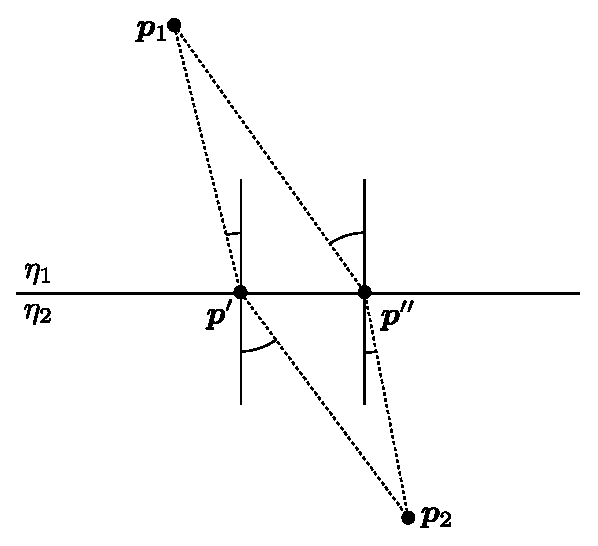
\includegraphics[width=0.5\linewidth]{Pictures/chap08/Fermatsprinciple.eps}
              \caption{斯涅尔定律的推导。斯涅尔定律可以用费马原理推导出,
                  即光在两点间传播时会遵循时间最短的路径。
                  因而两种介质边界上的折射角$\theta$可被证明最小化了
                  从点$\bm{p}_1$到点$\bm{p}'$的耗时加上从该点到点$\bm{p}_2$的耗时。}
              \label{fig:8.25}
          \end{figure}
    \item \circlethree 阅读论文\citet{10.1109/38.62695}与\citet{10.1145/192161.192204},
          并运用其描述的一些技术修改pbrt以对光的偏振效应建模。
          构建场景并渲染它们的图像以说明当精确建模偏振时产生的显著差异。
    \item \circlethree 用含有大量镜像微面的粗糙平面构造一个含有真实几何模型的场景
          \footnote{必须用面光源而不是点光源或定向光源,因为镜像曲面中看到的这些光源有细微差异。
              对于pbrt所用的光传输算法,镜像曲面中的无穷小点光源是永远不可见的。
              这是光线追踪渲染器的典型局限性且实践中通常不会带来麻烦。}。
          把相机置于场景中使得每个像素区域内都有非常大量的微面,
          用成百上千的像素样本来渲染该场景图像。比较使用平坦曲面与基于微面的BRDF模型的结果。
          如果你尽量调整微面BRDF参数,你能让这两种方法匹配得多好?
          你能否构造例子,使得用正确的微面渲染的图像能因为更好地建模了掩模、
          自遮挡以及微面间的互反射效应而十分明显地更加逼真?
    \item \circlethree 扩展pbrt使其能更加精确地渲染像木材\citep{10.1145/1186822.1073254}、
          布料\citep{2003_sattler_egsr}或车漆\citep{guenther:05:carpaint}等有趣的曲面。
          比起使用pbrt为这些效果提供的现成反射函数,渲染展现出更好视觉效果的图像。
    \item \circlethree 实现基于仿真的方法来建模来自复杂微面的反射,例如\citet{10.1145/133994.134075}所述方法。
          修改pbrt使得你能提供对复杂曲面(例如布料、丝绒等)的微观几何的描述,
          从大量输入方向向几何体发射光线,并记录离开曲面的光线的分布和数量
          (你可能需要修改来自第\refchap{光传输I:表面反射}的\refvar{PathIntegrator}{}来
          确定出射光的分布)。若曲面是各向同性的,就在3D表中记录下分布,
          若是各向异性的就用4D表,然后用表格为渲染图像计算BRDF值。
          展示使用该方法时来自复杂曲面的有趣反射效应。
          探究表格大小和计算表中各项时所用的样本数目如何影响最终结果准确性。
    \item \circletwo 尽管pbrt特化了形状\refvar{Curve}{}来提供光线与参数曲线之间
          非常高效的相交(\refsec{曲线}),但它缺少头发的反射模型。
          从“扩展阅读”一节描述的模型中选择一个,
          例如\citet{10.1145/882262.882345}或\citet{10.1111/j.1467-8659.2011.01976.x},
          并在pbrt中实现它。寻找一个头发几何模型或用程序生成头发,并用你的实现渲染图像。
\end{enumerate}


\section{译者补充:两个微面分布函数的规范性证明}\label{sec:译者补充:两个微面分布函数的规范性证明}
本节中译者补充了\refeq{8.10}和\refeq{8.11}所给的
微面分布函数$D({\bm\omega}_{\mathrm{h}})$满足规范性要求的证明,即证明
\begin{align}\label{eq:8.ex-01}
    \int\limits_{H^2({\bm n})}D({\bm\omega}_{\mathrm{h}})\cos\theta_{\mathrm{h}}\mathrm{d}{\bm\omega}_{\mathrm{h}}=1\, .
\end{align}

为了简化证明过程,我们先证明以下积分式(其中$\alpha_x,\alpha_y>0$):
\begin{align}\label{eq:8.ex-02}
    \int_{\varphi_{\mathrm{h}}=0}^{2\pi}\frac{1}{2\pi\alpha_x\alpha_y\left(\frac{\cos^2\varphi_{\mathrm{h}}}{\alpha_x^2}+\frac{\sin^2\varphi_{\mathrm{h}}}{\alpha_y^2}\right)}\mathrm{d}\varphi_{\mathrm{h}}=1\, .
\end{align}
\begin{prove}
    \begin{align}
                                                         & \int_{\varphi_{\mathrm{h}}=0}^{2\pi}\frac{1}{2\pi\alpha_x\alpha_y\left(\frac{\cos^2\varphi_{\mathrm{h}}}{\alpha_x^2}+\frac{\sin^2\varphi_{\mathrm{h}}}{\alpha_y^2}\right)}\mathrm{d}\varphi_{\mathrm{h}}\nonumber \\
        =                                                & \int_{\varphi_{\mathrm{h}}=0}^{2\pi}\frac{\alpha_x\alpha_y}{2\pi(\alpha_x^2\sin^2\varphi_{\mathrm{h}}+\alpha_y^2\cos^2\varphi_{\mathrm{h}})}\mathrm{d}\varphi_{\mathrm{h}}\nonumber                               \\
        =                                                & \frac{\alpha_x\alpha_y}{2\pi}\int_{\varphi_{\mathrm{h}}=0}^{2\pi}\frac{1}{(\alpha_x^2\tan^2\varphi_{\mathrm{h}}+\alpha_y^2)\cos^2\varphi_{\mathrm{h}}}\mathrm{d}\varphi_{\mathrm{h}}\nonumber                     \\
        =                                                & \frac{\alpha_x\alpha_y}{\pi}\int_{\varphi_{\mathrm{h}}=0}^{\pi}\frac{1}{\alpha_x^2\tan^2\varphi_{\mathrm{h}}+\alpha_y^2}\mathrm{d}\tan\varphi_{\mathrm{h}}\nonumber                                               \\
        =                                                & \frac{\alpha_x\alpha_y}{\pi}\int_{\varphi_{\mathrm{h}}=-\frac{\pi}{2}}^{\frac{\pi}{2}}\frac{1}{\alpha_x^2\tan^2\varphi_{\mathrm{h}}+\alpha_y^2}\mathrm{d}\tan\varphi_{\mathrm{h}}\nonumber                        \\
        \xlongequal{\text{令}t=\tan\varphi_{\mathrm{h}}} & \frac{\alpha_x\alpha_y}{\pi}\int_{t=-\infty}^{+\infty}\frac{1}{\alpha_x^2t^2+\alpha_y^2}\mathrm{d}t\nonumber                                                                                                      \\
        =                                                & \frac{1}{\pi}\int_{t=-\infty}^{+\infty}\frac{1}{\left(\frac{\alpha_xt}{\alpha_y}\right)^2+1}\mathrm{d}\frac{\alpha_xt}{\alpha_y}\nonumber                                                                         \\
        =                                                & \frac{1}{\pi}\arctan\frac{\alpha_xt}{\alpha_y}\bigg|_{t=-\infty}^{+\infty}\nonumber                                                                                                                               \\
        =                                                & 1\, .
    \end{align}
\end{prove}

接下来证明各向异性的Beckmann-Spizzichino模型即\refeq{8.10}满足规范性。
\begin{prove}
    设
    \begin{align}\label{eq:8.ex-03}
        \beta=\frac{\cos^2\varphi_{\mathrm{h}}}{\alpha_x^2}+\frac{\sin^2\varphi_{\mathrm{h}}}{\alpha_y^2}>0\quad(\alpha_x,\alpha_y>0)\, .
    \end{align}
    利用上述变量简化积分并结合\refeq{8.ex-02},可得
    \begin{align}
          & \int\limits_{H^2({\bm n})}D({\bm\omega}_{\mathrm{h}})\cos\theta_{\mathrm{h}}\mathrm{d}{\bm\omega}_{\mathrm{h}}\nonumber                                                                                                                                                                                                                                                         \\
        = & \int\limits_{H^2({\bm n})}\frac{\mathrm{e}^{-\left(\frac{\cos^2\varphi_{\mathrm{h}}}{\alpha_x^2}+\frac{\sin^2\varphi_{\mathrm{h}}}{\alpha_y^2}\right)\tan^2\theta_{\mathrm{h}}}}{\pi\alpha_x\alpha_y\cos^4\theta_{\mathrm{h}}}\cos\theta_{\mathrm{h}}\mathrm{d}{\bm\omega}_{\mathrm{h}}\nonumber                                                                                \\
        = & \int_{\varphi_{\mathrm{h}}=0}^{2\pi}\int_{\theta_{\mathrm{h}}=0}^{\frac{\pi}{2}}\frac{\mathrm{e}^{-\left(\frac{\cos^2\varphi_{\mathrm{h}}}{\alpha_x^2}+\frac{\sin^2\varphi_{\mathrm{h}}}{\alpha_y^2}\right)\tan^2\theta_{\mathrm{h}}}}{\pi\alpha_x\alpha_y\cos^3\theta_{\mathrm{h}}}\sin\theta_{\mathrm{h}}\mathrm{d}\theta_{\mathrm{h}}\mathrm{d}\varphi_{\mathrm{h}}\nonumber \\
        = & \int_{\varphi_{\mathrm{h}}=0}^{2\pi}\int_{\theta_{\mathrm{h}}=0}^{\frac{\pi}{2}}\frac{\tan\theta_{\mathrm{h}}}{\pi\alpha_x\alpha_y\cos^2\theta_{\mathrm{h}}}\mathrm{e}^{-\beta \tan^2\theta_{\mathrm{h}}}\mathrm{d}\theta_{\mathrm{h}}\mathrm{d}\varphi_{\mathrm{h}}\nonumber                                                                                                   \\
        = & \int_{\varphi_{\mathrm{h}}=0}^{2\pi}\int_{\theta_{\mathrm{h}}=0}^{\frac{\pi}{2}}\frac{-1}{2\pi\alpha_x\alpha_y\beta}\mathrm{d}\mathrm{e}^{-\beta \tan^2\theta_{\mathrm{h}}}\mathrm{d}\varphi_{\mathrm{h}}\nonumber                                                                                                                                                              \\
        = & \int_{\varphi_{\mathrm{h}}=0}^{2\pi}\frac{-1}{2\pi\alpha_x\alpha_y\beta}\left(\mathrm{e}^{-\beta \tan^2\theta_{\mathrm{h}}}\bigg|_{\theta_{\mathrm{h}}=0}^{\frac{\pi}{2}}\right)\mathrm{d}\varphi_{\mathrm{h}}\nonumber                                                                                                                                                         \\
        = & \int_{\varphi_{\mathrm{h}}=0}^{2\pi}\frac{1}{2\pi\alpha_x\alpha_y\beta}\mathrm{d}\varphi_{\mathrm{h}}\nonumber                                                                                                                                                                                                                                                                  \\
        = & 1\, .
    \end{align}
\end{prove}

Trowbridge-Reitz模型即\refeq{8.11}的证明是类似的。
\begin{prove}
    同样按\refeq{8.ex-03}设好$\beta$,结合\refeq{8.ex-02},可得
    \begin{align}
                                                                 & \int\limits_{H^2({\bm n})}D({\bm\omega}_{\mathrm{h}})\cos\theta_{\mathrm{h}}\mathrm{d}{\bm\omega}_{\mathrm{h}}\nonumber                                                                                                                                                                                                                                                            \\
        =                                                        & \int\limits_{H^2({\bm n})}\frac{1}{\pi\alpha_x\alpha_y\left(1+\left(\frac{\cos^2\varphi_{\mathrm{h}}}{\alpha_x^2}+\frac{\sin^2\varphi_{\mathrm{h}}}{\alpha_y^2}\right)\tan^2\theta_{\mathrm{h}}\right)^2\cos^4\theta_{\mathrm{h}}}\cos\theta_{\mathrm{h}}\mathrm{d}{\bm\omega}_{\mathrm{h}}\nonumber                                                                               \\
        =                                                        & \int_{\varphi_{\mathrm{h}}=0}^{2\pi}\int_{\theta_{\mathrm{h}}=0}^{\frac{\pi}{2}}\frac{\sin\theta_{\mathrm{h}}}{\pi\alpha_x\alpha_y\left(1+\left(\frac{\cos^2\varphi_{\mathrm{h}}}{\alpha_x^2}+\frac{\sin^2\varphi_{\mathrm{h}}}{\alpha_y^2}\right)\tan^2\theta_{\mathrm{h}}\right)^2\cos^3\theta_{\mathrm{h}}}\mathrm{d}\theta_{\mathrm{h}}\mathrm{d}\varphi_{\mathrm{h}}\nonumber \\
        =                                                        & \int_{\varphi_{\mathrm{h}}=0}^{2\pi}\int_{\theta_{\mathrm{h}}=0}^{\frac{\pi}{2}}\frac{\tan\theta_{\mathrm{h}}}{\pi\alpha_x\alpha_y(1+\beta\tan^2\theta_{\mathrm{h}})^2\cos^2\theta_{\mathrm{h}}}\mathrm{d}\theta_{\mathrm{h}}\mathrm{d}\varphi_{\mathrm{h}}\nonumber                                                                                                               \\
        =                                                        & \int_{\varphi_{\mathrm{h}}=0}^{2\pi}\int_{\theta_{\mathrm{h}}=0}^{\frac{\pi}{2}}\frac{1}{2\pi\alpha_x\alpha_y\beta(1+\beta\tan^2\theta_{\mathrm{h}})^2}\mathrm{d}(\beta\tan^2\theta_{\mathrm{h}})\mathrm{d}\varphi_{\mathrm{h}}\nonumber                                                                                                                                           \\
        \xlongequal{\text{令}u=1+\beta\tan^2\theta_{\mathrm{h}}} & \int_{\varphi_{\mathrm{h}}=0}^{2\pi}\int_{u=1}^{+\infty}\frac{1}{2\pi\alpha_x\alpha_y\beta u^2}\mathrm{d}u\mathrm{d}\varphi_{\mathrm{h}}\nonumber                                                                                                                                                                                                                                  \\
        =                                                        & \int_{\varphi_{\mathrm{h}}=0}^{2\pi}\int_{u=1}^{+\infty}\frac{-1}{2\pi\alpha_x\alpha_y\beta}\mathrm{d}u^{-1}\mathrm{d}\varphi_{\mathrm{h}}\nonumber                                                                                                                                                                                                                                \\
        =                                                        & \int_{\varphi_{\mathrm{h}}=0}^{2\pi}\frac{-1}{2\pi\alpha_x\alpha_y\beta}\left(\frac{1}{u}\bigg|_{u=1}^{+\infty}\right)\mathrm{d}\varphi_{\mathrm{h}}\nonumber                                                                                                                                                                                                                      \\
        =                                                        & \int_{\varphi_{\mathrm{h}}=0}^{2\pi}\frac{1}{2\pi\alpha_x\alpha_y\beta}\mathrm{d}\varphi_{\mathrm{h}}\nonumber                                                                                                                                                                                                                                                                     \\
        =                                                        & 1\, .
    \end{align}
\end{prove}

\section{译者补充:经典电磁理论下的光学基础}\label{sec:译者补充:经典电磁理论下的光学基础}
\begin{remark}
    本节内容不是原书内容,而是译者根据《Optics》\citep{hecht2016optics}
    补充并参考\citet{OpticsChinese}翻译的,请酌情参考和斧正。
    本节内容只简要介绍相关基础概念和结论,
    并不像正式的物理和光学教材那样严谨,请读者批判性地看待本节内容。
    本节要求读者具备较好的微积分与电磁理论知识储备。
    此外读者需注意,本节遵循有关内容惯例采用右手坐标系,
    与正文pbrt采用的左手坐标系不同。
\end{remark}

\subsection{波动}\label{sub:波动}
光的本质是什么?光是波动现象还是粒子现象?
这个问题非常复杂。早在二十世纪,物理学家们就已经发现,
光的电磁理论的经典结论在微观层级上完全不成立。
然而当我们站在通常的大尺度视角下,电磁波及其经典理论已经够用了。
为了打好基础,我们从波的数学描述说起,它也适用于一切物理波。

\subsubsection*{一维波}
行进中的\keyindex{波}{wave}{}的一个本质特性是,
它是传播波的\keyindex{介质}{medium}{}的自持\keyindex{扰动}{disturbance}{}。
\keyindex{机械波}{mechanical wave}{wave\ 波}是
我们最熟悉的波,例如琴弦上的波、液体表面的波以及
空气中的\keyindex{声波}{sound wave}{wave\ 波}。
波还有纵波、横波之分。介质在波动方向上位移的是\keyindex{纵波}{longitudinal wave}{wave\ 波}。
介质位移的方向垂直于波动方向的是\keyindex{横波}{transverse wave}{wave\ 波}。
例如,声波是纵波;琴弦上的波、电磁波是横波。

波区别于粒子流的几个关键特征之一是,
扰动在前进,但实物介质并不前进。
就像风吹起滚滚麦浪,但麦穗只是原地摇摆。
\begin{figure}[htbp]
    \centering
    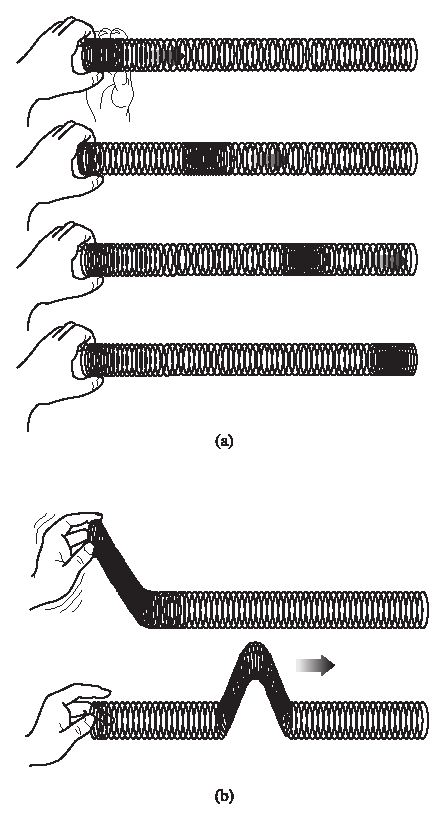
\includegraphics[width=0.65\linewidth]{Pictures/chap08/longitudinalAndTransverseWave.eps}
    \caption{弹簧中的(a)纵波;(b)横波。}
    \label{fig:08ex02.0201}
\end{figure}

我们暂不追究扰动的本质,而专注研究描述波动的方程应该具备怎样的形式。
设某个这样的扰动$\psi$以恒定速度$v$沿正$x$方向运动。
既然扰动在运动,则它必然是位置和时间的函数:
\begin{align}
    \psi(x,t)=f(x,t)\, ,
\end{align}
其中$f(x,t)$对应于某个具体函数或波形。
如\reffig{08ex02.0203}(a)所示,一个脉冲在静止坐标系$S$中以速度$v$运动。
我们取定任意时刻$t$即可得到那个时刻波的\keyindex{剖面}{profile}{},
就像脉冲经过时给它“拍照”。例如$t=0$有
\begin{align}
    \psi(x,t)\bigg|_{t=0}=f(x,0)=f(x)
\end{align}
表示0时刻波的剖面。
\begin{figure}[htb]
    \centering
    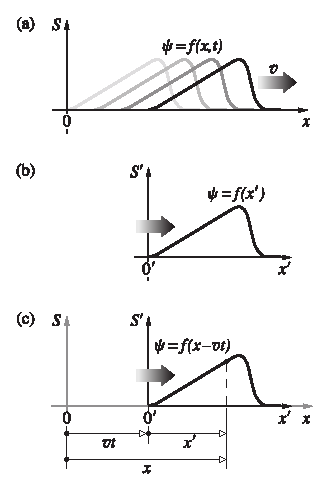
\includegraphics[width=0.5\linewidth]{Pictures/chap08/MovingReferenceFrame.eps}
    \caption{运动参考系。}
    \label{fig:08ex02.0203}
\end{figure}

现在,我们先只考虑传播时形状不变的波。
在一段时间$t$后,脉冲沿$x$轴前进了距离$vt$,其余不变。
如\reffig{08ex02.0203}(b),我们引入新坐标系$S'$并与脉冲以相同速度$v$运动。
则在该坐标系中$\psi$不再是时间的函数,而是静止不变的剖面,即
\begin{align}
    \psi=f(x')\, ,
\end{align}
这意味着坐标系$S'$中的扰动在任意时刻$t$的形状,
都和$S$中$t=0$时两者具有同一原点时扰动的形状相同,如\reffig{08ex02.0203}(c)所示。
为了将上式改写为$S$中某静止观察者描述的形式,我们利用
\begin{align}
    x'=x-vt
\end{align}
得到
\begin{align}
    \psi(x,t)=f(x-vt)\, .
\end{align}
上式是一维\keyindex{波函数}{wave function}{wave\ 波}的最一般形式。
它描述了一个具有所需剖面形状$f(x)$的波,它以速度$v>0$沿正$x$方向运动。
相似地,如果波向负$x$方向运动,则上式应改写为
\begin{align}
    \psi(x,t)=f(x+vt)\, .
\end{align}
总之变量$x$和$t$一定作为一个整体变量$x\mp vt$出现。

\subsubsection*{波动微分方程}
接下来我们推导一维波动方程的形式,把$\psi(x,t)$对空间与时间的依赖关系联系起来。注意到
\begin{align}
    \frac{\partial x'}{\partial x}=\frac{\partial (x\mp vt)}{\partial x}=1\, ,
\end{align}
以及
\begin{align}
    \frac{\partial x'}{\partial t}=\mp v\, ,
\end{align}
所以$\psi(x,t)$在$t$恒定时对$x$的偏微分为
\begin{align}
    \frac{\partial \psi}{\partial x}
    =\frac{\partial f}{\partial x}
    =\frac{\partial f}{\partial x'}\frac{\partial x'}{\partial x}
    =\frac{\partial f}{\partial x'}\, .
\end{align}
而在$x$恒定时$\psi(x,t)$对$t$的偏微分为
\begin{align}
    \frac{\partial \psi}{\partial t}
    =\frac{\partial f}{\partial t}
    =\frac{\partial f}{\partial x'}\frac{\partial x'}{\partial t}
    =\mp v\frac{\partial f}{\partial x'}
    =\mp v\frac{\partial \psi}{\partial x}\, .
\end{align}
上式表明$\psi$对$x$和$t$的变化率只差一个常系数。
继续求$\psi$的二阶偏微分有
\begin{align}
    \frac{\partial^2 \psi}{\partial x^2}
    =\frac{\partial}{\partial x}\left(\frac{\partial \psi}{\partial x}\right)
    =\frac{\partial}{\partial x}\left(\frac{\partial f}{\partial x'}\right)
    =\frac{\partial}{\partial x'}\left(\frac{\partial f}{\partial x'}\right)\frac{\partial x'}{\partial x}
    =\frac{\partial^2 f}{\partial x'^2}\, ,
\end{align}
并进一步得到
\begin{align}
    \frac{\partial^2 \psi}{\partial t^2}
    = & \frac{\partial}{\partial t}\left(\frac{\partial \psi}{\partial t}\right)
    =\frac{\partial}{\partial t}\left(\mp v\frac{\partial f}{\partial x'}\right)\nonumber    \\
    = & \mp v\frac{\partial}{\partial x'}\left(\frac{\partial f}{\partial t}\right)
    =\mp v\frac{\partial}{\partial x'}\left(\frac{\partial \psi}{\partial t}\right)\nonumber \\
    = & \mp v\frac{\partial}{\partial x'}\left(\mp v\frac{\partial f}{\partial x'}\right)
    =v^2\frac{\partial^2 f}{\partial x'^2}\nonumber                                          \\
    = & v^2\frac{\partial^2 \psi}{\partial x^2}\, .
\end{align}
整理上式即
\begin{definition}[一维\keyindex{波动微分方程}{differential wave equation}{equation\ 方程}]
    \begin{align}
        \frac{\partial^2 \psi}{\partial x^2}=\frac{1}{v^2}\frac{\partial^2 \psi}{\partial t^2}\, .
    \end{align}
\end{definition}
注意上式是一个\keyindex{齐次微分方程}{homogeneous differential equation}{equation\ 方程},
没有仅含独立变量的项(例如一份“力”或“源”),
所以描述的是\keyindex{无阻尼系统}{undamped system}{system\ 系统}。
这意味着若$\psi$是方程的解,则它乘以任意倍数后也是解。
反之,若一个波函数是上述方程的解,则它将是$x\mp vt$的函数,
且可以对$x$和$t$求得非平凡的二阶微分。

\subsubsection*{谐波}
最简单的波形是正弦或余弦曲线。它可以称作
\keyindex{正弦波}{sinusoidal wave}{wave\ 波}、
\keyindex{简谐波}{simple harmonic wave}{wave\ 波}
或\keyindex{谐波}{harmonic wave}{wave\ 波}。
任何波形都可以由谐波叠加合成。

我们为谐波波形选定为以下简单函数:
\begin{align}
    \psi(x,t)\bigg|_{t=0}=\psi(x)=f(x)=A\sin kx\, ,
\end{align}
其中常数$k>0$称作\keyindex{传播数}{propagation number}{},
$kx$这个整体是无量纲的。$\psi(x)$的最大值$A>0$称作波的\keyindex{振幅}{amplitude}{}。
将上式中的$x$替换为$x-vt$,改写成以速度$v$沿正$x$方向前进的波:
\begin{align}
    \psi(x,t)=A\sin k(x-vt) = f(x-vt)\, .
\end{align}
显然它是波动微分方程的一个解。该波在空间和时间中都具有周期性。
它的\keyindex{空间周期}{spatial period}{period\ 周期}
称作\keyindex{波长}{wavelength}{},表示每个波的长度,记作$\lambda$.
当$x$大小增减$\lambda$,$\psi$应不变:
\begin{align}
    \psi(x,t)=\psi(x\pm\lambda,t)\, .
\end{align}
这对应了正弦函数自变量改变$\pm2\pi$,由于$k>0,\ \lambda>0$,所以
\begin{align}
    \lambda=\frac{2\pi}{k}\, .
\end{align}

类似地,$\psi$的\keyindex{时间周期}{temporal period}{period\ 周期}记作$\tau$,
可简称\keyindex{周期}{period}{},即一个完整的波经过一静止观察者的时间。
它对应了波在时间上的重复行为:
\begin{align}
    \psi(x,t)=\psi(x,t\pm\tau)\, .
\end{align}
由此我们容易推出
\begin{align}
    kv\tau=2\pi\, ,
\end{align}
以及
\begin{align}
    \tau=\frac{\lambda}{v}\, .
\end{align}

周期的倒数称作\keyindex{时间频率}{temporal frequency}{frequency\ 频率},
可简称\keyindex{频率}{frequency}{},记作$\nu$,即单位时间里波的个数:
\begin{align}
    \nu=\frac{1}{\tau}\, ,
\end{align}
其单位为\keyindex{赫兹}{Hertz}{}(简写为Hz),即每秒周数。
结合前述定义,不难发现\keyindex{波速}{speed}{}
$v$满足\sidenote{注意$v$是英语字母,$\nu$是希腊字母。}
\begin{align}
    v=\nu\lambda\, .
\end{align}

此外我们还定义\keyindex{时间角频率}{angular temporal frequency}{frequency\ 频率}为
\begin{align}
    \omega=\frac{2\pi}{\tau}=2\pi\nu=kv\, ,
\end{align}
可简称为\keyindex{角频率}{angular frequency}{frequency\ 频率},单位为弧度每秒(rad/s)。

此外,\keyindex{空间频率}{spatial frequency}{frequency\ 频率},
也称\keyindex{波数}{wavenumber}{},定义为
\begin{align}
    \kappa=\frac{1}{\lambda}\, ,
\end{align}
即单位长度中波的数目,单位为$\mathrm{m}^{-1}$.

以上所有概念也适用于非谐波,只要它是由单个剖面元规则重复构成的。

利用以上定义,我们可以写出以下常见而等价的谐波表达式:
\begin{align}
    \psi= & A\sin k(x\mp vt)\, ,                                          \\
    \psi= & A\sin (kx\mp\omega t)\, ,                                     \\
    \psi= & A\sin 2\pi\left(\frac{x}{\lambda}\mp\frac{t}{\tau}\right)\, , \\
    \psi= & A\sin 2\pi(\kappa x\mp\nu t)\, ,                              \\
    \psi= & A\sin 2\pi\nu\left(\frac{x}{v}\mp t\right)\, ,
\end{align}
其中前两个最为常用,你甚至可以改用余弦函数来表示(后文就有)。
注意到这些理想化波的$x$和$t$没有取值范围限制,
又具有单一恒定频率,所以称作是\keyindex{单色的}{monochromatic}{}
或\keyindex{单能量的}{monoenergetic}{}。
但真实的波无法无限回溯到$t=-\infty$,所以不会是严格的单色波,而是含有一个频率范围。
若这个频段很窄,则称该波是\keyindex{准单色的}{quasimonochromatic}{}。

\subsubsection*{相位与相速度}
考察任一谐波,如
\begin{align}
    \psi(x,t)= & A\sin (kx-\omega t)\, ,
\end{align}
称正弦函数的整个输入值为波的\keyindex{相位}{phase}{},记作
\begin{align}
    \varphi=kx-\omega t\, .
\end{align}
更普遍地,对于谐波
\begin{align}
    \psi(x,t)= & A\sin (kx-\omega t+\varepsilon)\, ,
\end{align}
其相位为
\begin{align}
    \varphi=kx-\omega t+\varepsilon\, ,
\end{align}
其中$t=0$且$x=0$时的相位$\varepsilon$称作\keyindex{初相}{initial phase}{}。

根据相位定义,可知当$x$恒定时,相位对时间的变化率为
\begin{align}
    \left|\left(\frac{\partial\varphi}{\partial t}\right)_x\right|=\omega\, .
\end{align}
当$t$恒定时,相位对距离的变化率为
\begin{align}
    \left|\left(\frac{\partial\varphi}{\partial x}\right)_t\right|=k\, .
\end{align}
利用链式法则等微分知识,可推得
\begin{align}
    \left(\frac{\partial x}{\partial t}\right)_{\varphi}
    =-\displaystyle\frac{(\partial\varphi/\partial t)_x}
    {(\partial\varphi/\partial x)_t}
    =\pm\frac{\omega}{k}=\pm v\, .
\end{align}
上式最左边表示相位恒定状态的传播速度,称作波的\keyindex{相速度}{phase velocity}{}。
这里$v>0$,当波朝着正$x$方向运动时,则相速度取正号,反之则取负号。

\subsubsection*{叠加原理}
波动微分方程揭示了波一个明显区别于经典粒子流的性质:
\begin{theorem}[\keyindex{叠加原理}{superposition principle}{}]
    若$\psi_1$和$\psi_2$是同一波动方程的两个不同的解,
    则叠加它们的$\psi_1+\psi_2$也是一个解。
\end{theorem}
这意味着两个波到达同一片空间时会发生重叠,
简单地与另一方相加(相减),而不会永久瓦解其中某个波。
重叠区域内每一点的合扰动是该位置上单个成分波的代数之和。
在穿过共存区域后,每个波会继续前进离开,不受这次干扰。
注意这里我们讨论的是最为广泛的波的线性叠加,
暂不考虑极端情况下波的振幅大到以非线性方式驱动介质。

\begin{figure}[htb]
    \centering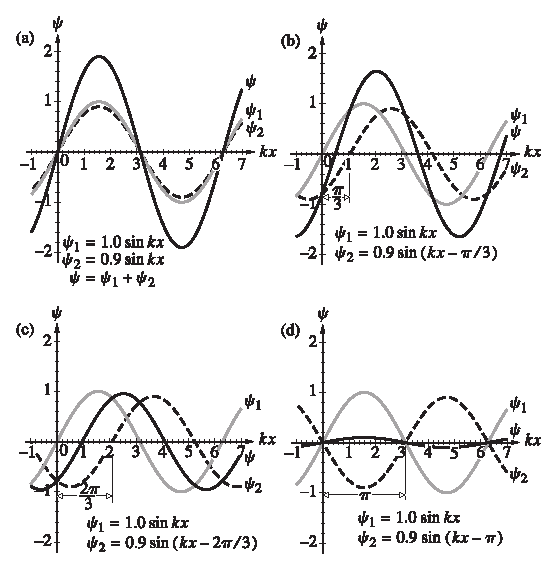
\includegraphics[width=0.9\linewidth]{Pictures/chap08/SuperpositionOfTwoSinusoids.eps}
    \caption{两个正弦波$\psi_1$和$\psi_2$的叠加,振幅分别为$A_1=1.0$和$A_2=0.9$.
        (a)$\psi_1$和$\psi_2$同相。(b)$\psi_1$领先$\psi_2$相角$\displaystyle\frac{\pi}{3}$.
        (c)$\psi_1$领先$\psi_2$相角$\displaystyle\frac{2\pi}{3}$.
        (d)$\psi_1$和$\psi_2$相位相差$\pi$,几乎要相互抵消。}
    \label{fig:08ex02.0216}
\end{figure}
\reffig{08ex02.0216}展示了两个振幅十分接近的波叠加后的结果与它们之间相位差的关系。
\reffig{08ex02.0216}(a)中两个波相位差为零,称为\keyindex{同相}{in-phase}{}。
它们互相加强,振幅增大,频率和波长不变。随着相位差增大,合成波振幅减小,
直到\reffig{08ex02.0216}(d)中相位差达到$\pi$,合成波几乎消失,
此时称两个波\keyindex{异相}{out-of-phase}{}
$180^\circ$.
异相波倾向于互相抵消的现象使得这整类现象被称作\keyindex{干涉}{interference}{}。

\subsubsection*{波的复数表示}
谐波所含的三角函数不便于数学处理,因此我们引入更方便的复数表示方法
\sidenote{本节复数等数学符号暂时遵循参考文献的记法。}。
\keyindex{复数}{complex number}{}
$\widetilde{z}$形如
\begin{align}
    \widetilde{z}=x+\mathrm{i}y=r(\cos\theta+\mathrm{i}\sin\theta)=r\mathrm{e}^{\mathrm{i}\theta}\, ,
\end{align}
其中\keyindex{虚数单位}{imaginary unit}{}
$\mathrm{i}=\sqrt{-1}$.
实数$x$和$y$分别为$\widetilde{z}$的\keyindex{实部}{real part}{complex number\ 复数}
和\keyindex{虚部}{imaginary part}{complex number\ 复数};
实数$r\ge0$和$\theta$分别为$\widetilde{z}$的\keyindex{长度}{magnitude}{complex number\ 复数}
和\keyindex{相角}{phase angle}{complex number\ 复数};
长度也常记作$|\widetilde{z}|$,称为复数的\keyindex{模}{modulus}{complex number\ 复数}
或\keyindex{绝对值}{absolute value}{complex number\ 复数}。

本节中,复数的\keyindex{复共轭}{complex conjugate}{}用星号表示,即
\begin{align}
    \widetilde{z}^*=(x+\mathrm{i}y)^*=x-\mathrm{i}y
    =r(\cos\theta-\mathrm{i}\sin\theta)=r\mathrm{e}^{-\mathrm{i}\theta}\, .
\end{align}
于是复数的实部和虚部可以表示为
\begin{align}
    \mathrm{Re}(\widetilde{z}) & =\frac{1}{2}(\widetilde{z}+\widetilde{z}^*)=r\cos\theta\, ,           \\
    \mathrm{Im}(\widetilde{z}) & =\frac{1}{2\mathrm{i}}(\widetilde{z}-\widetilde{z}^*)=r\sin\theta\, .
\end{align}
我们习惯上选用实部来描述谐波,即
\begin{align}
    \psi(x,t)=\mathrm{Re}[A\mathrm{e}^{\mathrm{i}(\omega t-kx+\varepsilon)}]\, ,
\end{align}
它等价于
\begin{align}
    \psi(x,t)=A\cos(\omega t-kx+\varepsilon)\, .
\end{align}
于是为了方便,在后文中我们略去实部记号把波函数简写为
\begin{align}
    \psi(x,t)=A\mathrm{e}^{\mathrm{i}(\omega t-kx+\varepsilon)}=A\mathrm{e}^{\mathrm{i}\varphi}\, ,
\end{align}
并借助复数运算法则(尤其是复指数乘除法的简便性)来进行计算,
只在要表示实际波时才取回实部。

要注意的是,波被表示为复数函数后,若参与了运算,
则只有当这些运算仅限于加减法、乘或除以一个实数,
或对一个实数变量进行微分或积分,才能恢复其实部,否则结果是错误的。

\subsubsection*{平面波}
给定时刻的光波可以用其频率、振幅、传播方向等描述,
但这并没有告诉我们光扰动在一片延伸的空间内的更多信息。
为此我们已经在定义\ref{definition:wavefront}中
引入了\keyindex{波阵面}{wavefront}{}
的概念。本节将研究理想的平面波的数学表达
\sidenote{本节向量等数学符号暂时遵循参考文献的记法。}。

\begin{figure}[htbp]
    \centering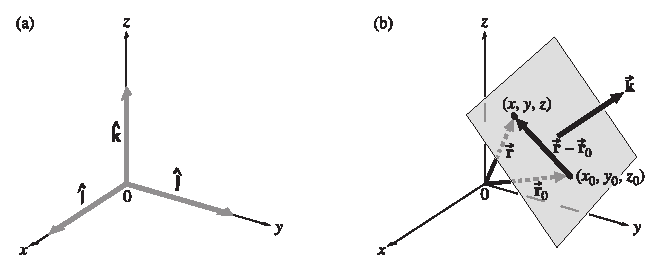
\includegraphics[width=\linewidth]{Pictures/chap08/CartesianUnitBasisVectors.eps}
    \caption{(a)直角坐标系单位基向量。(b)沿着$\vec{\mathbf{k}}$方向运动的平面波。}
    \label{fig:08ex02.0221}
\end{figure}
\keyindex{平面波}{plane wave}{wave\ 波}
是最简单的三维波了,其扰动的一切等相面构成一组平面,
且一般都垂直于传播方向。为此我们先给出平面的数学表达式:
如\reffig{08ex02.0221}(a)所示,对于直角坐标系中
的位置向量$\vec{\mathbf{r}}$,我们用三个坐标轴上的单位基向量来表示为
\begin{align}
    \vec{\mathbf{r}}=x\hat{\text{\sffamily\bfseries i}}+y\hat{\text{\sffamily\bfseries j}}+z\hat{\text{\sffamily\bfseries k}}\, .
\end{align}
它始于某个任意的原点$O$,止于点$(x,y,z)$,该点可以是空间中的任意位置。
类似地如\reffig{08ex02.0221}(b)所示,有
\begin{align}
    \vec{\mathbf{r}}-\vec{\mathbf{r}}_0
    =(x-x_0)\hat{\text{\sffamily\bfseries i}}+(y-y_0)\hat{\text{\sffamily\bfseries j}}+(z-z_0)\hat{\text{\sffamily\bfseries k}}\, .
\end{align}
我们令
\begin{align}
    (\vec{\mathbf{r}}-\vec{\mathbf{r}}_0)\cdot\vec{\mathbf{k}}=0\, ,
\end{align}
使向量$\vec{\mathbf{r}}-\vec{\mathbf{r}}_0$扫过
一垂直于$\vec{\mathbf{k}}$的平面,其端点$(x,y,z)$取一切允许的值。
设$\vec{\mathbf{k}}$为
\begin{align}
    \vec{\mathbf{k}}=k_x\hat{\text{\sffamily\bfseries i}}+k_y\hat{\text{\sffamily\bfseries j}}+k_z\hat{\text{\sffamily\bfseries k}}\, ,
\end{align}
则有
\begin{align}
    k_x(x-x_0)+k_y(y-y_0)+k_z(z-z_0)=0\, ,
\end{align}
即
\begin{align}
    k_xx+k_yy+k_zz=a\, ,
\end{align}
其中
\begin{align}
    a=k_xx_0+k_yy_0+k_zz_0=\text{常数}\, .
\end{align}
于是垂直于$\vec{\mathbf{k}}$的平面方程最简洁的表达形式为
\begin{align}
    \vec{\mathbf{k}}\cdot\vec{\mathbf{r}}=\text{常数}\, .
\end{align}
位置向量在$\vec{\mathbf{k}}$方向上的投影相同的所有点构成的轨迹即该平面。

\begin{figure}[htbp]
    \centering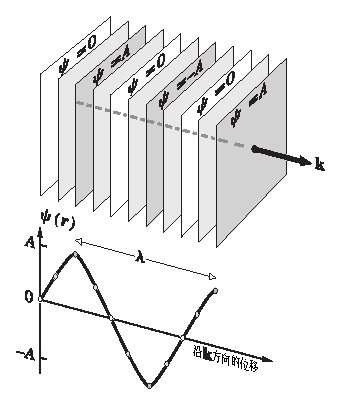
\includegraphics[width=0.5\linewidth]{Pictures/chap08/WavefrontsHarmonicPlaneWave.eps}
    \caption{平面简谐波的波阵面。}
    \label{fig:08ex02.0222}
\end{figure}
如\reffig{08ex02.0222},现在我们构建一组平面,
其上的$\psi(\vec{\mathbf{r}})$于空间中正弦地变化,即
\begin{align}
    \psi(\vec{\mathbf{r}})= & A\sin(\vec{\mathbf{k}}\cdot\vec{\mathbf{r}})\, ,                  \\
    \psi(\vec{\mathbf{r}})= & A\cos(\vec{\mathbf{k}}\cdot\vec{\mathbf{r}})\, ,                  \\
    \psi(\vec{\mathbf{r}})= & A\mathrm{e}^{\mathrm{i}\vec{\mathbf{k}}\cdot\vec{\mathbf{r}}}\, .
\end{align}
显然上面三个式子中,$\psi(\vec{\mathbf{r}})$都在
由$\vec{\mathbf{k}}\cdot\vec{\mathbf{r}}$取常数定义的每个平面上保持恒定。
沿着$\vec{\mathbf{k}}$方向位移$\lambda$后,$\psi$应当在空间中重复。
注意\reffig{08ex02.0222}中只画了无数平面中的若干个,
而平面本身也应无穷延伸,因为扰动充满整个空间。
当平面波在其波阵面上任意处均有相同“强度”时,
我们称其为\keyindex{均匀波}{homogeneous wave}{wave\ 波}。

总之,$\psi$在空间中的周期性可以表示为
\begin{align}
    \psi(\vec{\mathbf{r}})=\psi\left(\vec{\mathbf{r}}+\frac{\lambda}{k}\vec{\mathbf{k}}\right)\, ,
\end{align}
这里$\vec{\mathbf{k}}$也称作\keyindex{传播向量}{propagation vector}{vector\ 向量},
其大小$k$就是传播数\sidenote{类似地,在后文的记号中,如果我们主要想强调一个向量的大小,
则可能会记作同一字母的标量形式。读者联系上下文即可理解。}。
接着,为了使波运动起来,我们引入时间等变量,最终便得到
\begin{align}\label{eq:08ex02.DirectionCosines}
    \psi(\vec{\mathbf{r}},t)=A\mathrm{e}^{\mathrm{i}(\vec{\mathbf{k}}\cdot\vec{\mathbf{r}}\mp\omega t)}\, .
\end{align}
若$\alpha,\beta$和$\gamma$是$\vec{\mathbf{k}}$在直角坐标系下的方向余弦,则上式还可以写作
\begin{align}
    \psi(x,y,z,t)=A\mathrm{e}^{\mathrm{i}(k(\alpha x+\beta y+\gamma z)\mp\omega t)}
    =A\mathrm{e}^{\mathrm{i}k(\alpha x+\beta y+\gamma z\mp vt)}\, ,
\end{align}
注意
\begin{align}
    \alpha^2+\beta^2+\gamma^2=1\, .
\end{align}

\subsubsection*{三维波动微分方程}
像前文推导一维波动微分方程那样,我们可以
类似地用\refeq{08ex02.DirectionCosines}推导出
\begin{definition}[\keyindex{三维波动微分方程}{three-dimensional differential wave equation}{equation\ 方程}]
    \begin{align}\label{eq:08ex02.3d-differential-wave}
        \frac{\partial^2 \psi}{\partial x^2}+\frac{\partial^2 \psi}{\partial y^2}
        +\frac{\partial^2 \psi}{\partial z^2}=\frac{1}{v^2}\frac{\partial^2 \psi}{\partial t^2}\, .
    \end{align}
\end{definition}
注意上式中$x,y$和$z$是对称出现的。引入\keyindex{拉普拉斯算符}{Laplacian operator}{}
\begin{align}
    \nabla^2\equiv\frac{\partial^2}{\partial x^2}
    +\frac{\partial^2}{\partial y^2}+\frac{\partial^2}{\partial z^2}\, ,
\end{align}
则\refeq{08ex02.3d-differential-wave}简化为
\begin{align}
    \nabla^2\psi=\frac{1}{v^2}\frac{\partial^2 \psi}{\partial t^2}\, .
\end{align}
可以证明
\begin{align}
    \psi(\vec{\mathbf{r}},t)=C_1f\left(\frac{1}{k}\vec{\mathbf{k}}\cdot\vec{\mathbf{r}}-vt\right)
    +C_2g\left(\frac{1}{k}\vec{\mathbf{k}}\cdot\vec{\mathbf{r}}+vt\right)
\end{align}
均是上述波动微分方程的平面波解,其中$f$和$g$是二阶可微的任意函数
(不一定为简谐函数),$C_1$和$C_2$是常数。

\subsection{电磁理论}\label{sub:电磁理论}
在\keyindex{经典电动力学}{classical electrodynamics}{}
的图像中,电磁波是连续传递能量的。但更现代的\keyindex{量子电动力学}{quantum electrodynamics}{}
则用一种质量为零的基本“粒子”来描述电磁相互作用和能量传递,这种粒子称作\keyindex{光子}{photon}{}。
光以波的形式在空间中传播,但在发射和吸收时又显出粒子性,即二象性。
平均而言,我们可以把大量光子流的平均作用看作是经典电磁波,
但要清楚电磁波的表观连续性只是宏观世界的假象,事情并不简单。

\subsubsection*{电磁理论基本定律}
实验显示,即使是在真空中分开的\keyindex{电荷}{electric charge}{}
也仍受彼此的相互作用。我们想象每个电荷都被称作电场
的东西包围着,并假设每个电荷与它所沉浸于其中的电场直接相互作用。
\begin{definition}[\keyindex{电场}{electric field}{}]
    若一个点电荷$q$受到电场的力$\vec{\mathbf{F}}_E$,
    则它所在位置上的电场$\vec{\mathbf{E}}$就由
    \begin{align}
        \vec{\mathbf{F}}_E=q\cdot\vec{\mathbf{E}}
    \end{align}
    定义,电场强度单位为伏特/米(V/m)或牛顿/库仑(N/C)。
\end{definition}

\begin{remark}
    \keyindex{伏特}{volt}{}
    (伏)是电压和电势单位,得名于18至19世纪意大利物理学家
    亚历山德罗·朱塞佩·安东尼奥·阿纳斯塔西奥·伏特
    (Alessandro Giuseppe Antonio Anastasio Volta);
    \keyindex{库仑}{coulomb}{}
    (库)是电荷量单位,得名于18至19世纪法国物理学家夏尔·奥古斯丁·德·库仑
    (Charles-Augustin de Coulomb)。
\end{remark}

\begin{theorem}[\keyindex{库仑定律}{Coulomb's law}{}]
    真空中两个静止点电荷之间的相互作用力,
    称作\keyindex{静电力}{electrostatic force}{}
    或\keyindex{库仑力}{Coulomb force}{},
    其大小$F$与它们的电荷量$q_1$、$q_2$的乘积成正比,
    与它们的距离$r$的平方成反比,作用力的方向在
    它们的连线上;同性电荷相斥,异性电荷相吸。
    该定律的标量形式为
    \begin{align}
        F=k_e\frac{q_1q_2}{r^2}\,
    \end{align}
    其中比例系数$k_e$称作\keyindex{静电力常量}{electrostatic force constant}{}
    或\keyindex{库仑常量}{Coulomb's constant}{},取值为
    \begin{align}
        k_e=\frac{1}{4\pi\epsilon_0}=8.9875517862\times10^9\text{N}\cdot \text{m}^2/\text{C}^2\, ,
    \end{align}
    其中$\epsilon_0$为真空电容率。
\end{theorem}

此外,一个运动的电荷还会受到另一个力$\vec{\mathbf{F}}_M$,
称作\keyindex{洛伦兹力}{Lorentz force}{},
它与运动电荷的速度$\vec{\mathbf{v}}$成正比。
为此我们定义另一个场$\vec{\mathbf{B}}$:
\begin{definition}[\keyindex{磁场}{magnetic field}{}]
    它使得
    \begin{align}
        \vec{\mathbf{F}}_M=q\cdot\vec{\mathbf{v}}\times\vec{\mathbf{B}}\, .
    \end{align}
    $\vec{\mathbf{B}}$的大小称作\keyindex{磁感应}{magnetic induction}{}
    强度,单位为\keyindex{特斯拉}{tesla}{}
    (T)。
\end{definition}

\begin{remark}
    磁感应强度单位得名于19至20世纪塞尔维亚裔美国物理学家
    尼古拉·特斯拉(Nikola Tesla)。
\end{remark}

若电荷在既有电场又有磁场的空间区域内运动,
则会同时受到$\vec{\mathbf{F}}_E$和$\vec{\mathbf{F}}_M$两个力,
合力为$\vec{\mathbf{F}}=q\cdot\vec{\mathbf{E}}+q\cdot\vec{\mathbf{v}}\times\vec{\mathbf{B}}$.
后文我们将看到,随时间变化的磁场会产生电场,随时间变化的电场会产生磁场,
两者的互相依赖性是描述光的关键。

\subsubsection*{法拉第感应定律}
法拉第(迈克尔·法拉第(Michael Faraday),18至19世纪英国物理学家)
在线圈实验中发现了\keyindex{电磁感应}{electromagnetic induction}{}
现象,而“变化”是其最实质性的因素。

\begin{figure}[htbp]
    \centering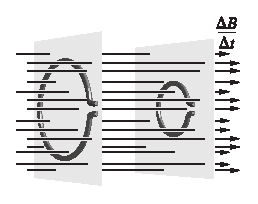
\includegraphics[width=0.4\linewidth]{Pictures/chap08/largerLoopGreaterEmf.eps}
    \caption{更大的环路通过更大的时变磁通量而产生更大的emf。}
    \label{fig:08ex02.0302}
\end{figure}
\begin{figure}[htbp]
    \centering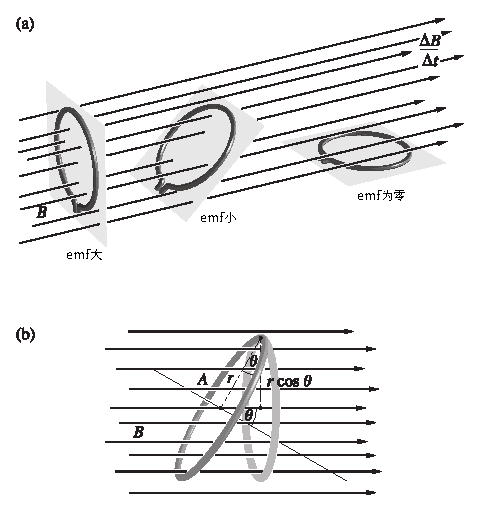
\includegraphics[width=0.75\linewidth]{Pictures/chap08/emfProportionalPerpendicularArea.eps}
    \caption{(a)感生电动势正比于磁场垂直穿过的面积。(b)垂直于磁场的面积随$\cos\theta$变化。}
    \label{fig:08ex02.0303}
\end{figure}

将一根磁铁插进线圈时,
线圈两端会有电压,称作\keyindex{感生电动势}{induced electromotive force}{}
(emf)\sidenote{作者强调,尽管英文中感生电动势被称作“force”,
但它并不是力,而是电压,所以会尽量用简称emf来避免误解。}。
该电动势的振幅依赖于磁铁运动速度,或者说依赖于穿过线圈的$B$的变化率,而不是$B$本身。
\reffig{08ex02.0302}中,同一变化的$B$场穿过两个不同导线环路,
大的环路两端有更大的感生电动势,即它正比于$B$场垂直穿过的环路面积$A$.
而\reffig{08ex02.0303}中,当环路变倾斜,则垂直于磁场的面积$A_{\perp}$
按$A\cos\theta$变化,其中$\theta$为倾角。当$\theta=90^\circ$时,
没有$B$场穿过环路,感生电动势为零。反之,当磁场恒定时,
感生电动势正比于磁场垂直穿过环路面积的变化率,此外它还正比于$B$.

总之,当$A_{\perp}$恒定时,$\mathrm{emf}\propto A_{\perp}\displaystyle\frac{\Delta B}{\Delta t}$;
当$B$恒定时,$\mathrm{emf}\propto B\displaystyle\frac{\Delta A_{\perp}}{\Delta t}$.
因此,感生电动势依赖于$A_{\perp}$与$B$乘积的变化率。
我们定义穿过导线环路的\keyindex{磁场通量}{flux of the magnetic field}{flux\ 通量}
为
\begin{align}
    \varPhi_M=B_{\perp}A=BA_{\perp}=BA\cos\theta\, ,
\end{align}
其单位为\keyindex{韦伯}{weber}{}
(Wb)\sidenote{得名于19世纪德国物理学家威廉·爱德华·韦伯(Wilhelm Eduard Weber)。}。

\begin{figure}[htbp]
    \centering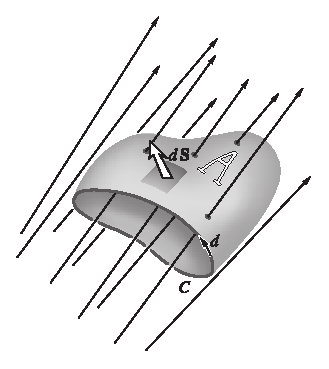
\includegraphics[width=0.5\linewidth]{Pictures/chap08/openAreaBoundedByClosedCurve.eps}
    \caption{$\vec{\mathbf{B}}$场穿过以闭合曲线$C$为边界的非闭合曲面$A$.}
    \label{fig:08ex02.0304}
\end{figure}

如\reffig{08ex02.0304},更一般地,$\vec{\mathbf{B}}$场可能在空间中变化。
穿过导电环路包围的任意非闭合曲面$A$的磁场通量为
\begin{align}
    \varPhi_M=\iint\limits_A\vec{\mathbf{B}}\cdot\mathrm{d}\vec{\mathbf{S}}\, ,
\end{align}
其中$\mathrm{d}\vec{\mathbf{S}}$垂直于曲面朝外。环路上的感生电动势则为
\begin{align}
    \mathrm{emf}=-\frac{\mathrm{d}\varPhi_M}{\mathrm{d}t}\, ,
\end{align}
其中负号说明
\begin{theorem}[\keyindex{楞次定律}{Lenz's law}{}]
    感生电动势想要驱动的感生电流,其对应的感生磁场总是想阻碍原先引发它的磁通量的变化。
\end{theorem}

任何一个场中沿着一条闭合曲线的路径积分叫做
该场的\keyindex{环量}{circulation}{}。
电动势也是一种电势差,即单位电荷的电势能之差,
也对应着对单位电荷做的功,或者说对应着电场乘以距离。
电动势只随电场出现:
\begin{align}
    \mathrm{emf}=\oint\limits_C\vec{\mathbf{E}}\cdot\mathrm{d}\vec{\mathbf{\ell}}\, ,
\end{align}
其中积分沿着对应于环路的闭合曲线$C$进行。
联立以上三式可得
\begin{theorem}[\keyindex{法拉第电磁感应定律}{Faraday's law of electromagnetic induction}{}]
    \begin{align}
        \oint\limits_C\vec{\mathbf{E}}\cdot\mathrm{d}\vec{\mathbf{\ell}}
        =-\frac{\mathrm{d}}{\mathrm{d}t}\iint\limits_A\vec{\mathbf{B}}\cdot\mathrm{d}\vec{\mathbf{S}}\, .
    \end{align}
\end{theorem}
上式除了积分路径$C$外就别无其他物理环路了。
$C$对于是否选在导体内外或附近也没有任何要求。
该式中的电场仅由时变的磁场产生,没有电荷作为电场的\keyindex{源}{source}{}
或\keyindex{汇}{sink}{},所以电场线均自身闭合形成环。

当我们感兴趣的是没有导线回路的空间中传播的电磁波时,
磁通量的变化是完全由$\vec{\mathbf{B}}$引起的,这时感应定律可重写为
\begin{align}
    \oint\limits_C\vec{\mathbf{E}}\cdot\mathrm{d}\vec{\mathbf{\ell}}
    =-\iint\limits_A\frac{\partial \vec{\mathbf{B}}}{\partial t}\cdot\mathrm{d}\vec{\mathbf{S}}\, .
\end{align}
上式表明一个随时间变化的磁场伴随有一个电场。

\subsubsection*{高斯定律}
电场的另一基本定律得名于18-19世纪德国数学家卡尔·弗里德里希·高斯(Carl Friedrich Gauss)。
高斯定律描述了电场通量和电荷之间的关系。
场和通量的概念都是从流体动力学引入的。
想象一个闭合曲面隔离出一团运动的流体,例如管道中充盈流动的水,
显然穿过它两个端面的体积流量大小相等,即单位时间内流进来和流出去的量相同。
此时全部表面上相加的流体净流量为零。
但如果有细针插进其中注入或吸走流体,即存在源或汇,则净流量将不为零。

这种概念同样适用于电场。如\reffig{08ex02.0307}所示,
考虑任意某电场中想象的封闭曲面$A$,则穿过$A$的
\keyindex{电场通量}{flux of the electric field}{flux\ 通量}
为
\begin{align}
    \varPhi_E=\oiint\limits_A\vec{\mathbf{E}}\cdot\mathrm{d}\vec{\mathbf{S}}\, ,
\end{align}
其中带圈的二重积分号强调积分曲面是封闭的,$\mathrm{d}\vec{\mathbf{S}}$垂直于曲面朝外。
当封闭曲面包围的区域内没有电场的源或汇时,电场通量等于零。
\begin{figure}[htbp]
    \centering
    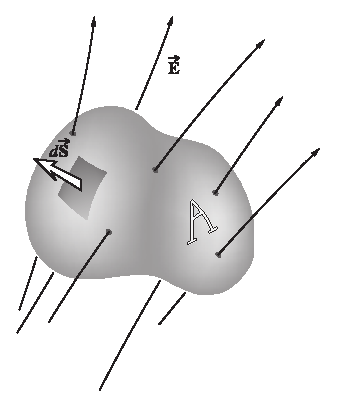
\includegraphics[width=0.5\linewidth]{Pictures/chap08/GausssLawElectric.eps}
    \caption{穿过封闭区域$A$的电场$\vec{\mathbf{E}}$.}
    \label{fig:08ex02.0307}
\end{figure}

当区域内存在源或汇时,考虑任意以正电荷$q$为球心、半径为$r$的球面。
根据库仑定律,该正电荷的电场$\vec{\mathbf{E}}$在球面表面任意处的大小均为
\begin{align}
    E=\frac{1}{4\pi\epsilon_0}\frac{q}{r^2}\, ,
\end{align}
且都沿径向向外垂直于球面表面,即$\vec{\mathbf{E}}=\vec{\mathbf{E}}_\perp$.
于是
\begin{align}
    \varPhi_E=\oiint\limits_A\vec{\mathbf{E}}\cdot\mathrm{d}\vec{\mathbf{S}}
    =\oiint\limits_A E_\perp\mathrm{d}S
    =E\oiint\limits_A\mathrm{d}S=4\pi r^2E=\frac{q}{\epsilon_0}\, .
\end{align}
推广到区域内的多个电荷时,将上式累加即可:
\begin{align}
    \varPhi_E=\frac{1}{\epsilon_0}\sum q\, .
\end{align}
把电荷分布近似为连续分布,在$A$所包围的体积$V$内,
记电荷分布密度为$\rho$,则我们最终得到
\begin{theorem}[电场的\keyindex{高斯定律}{Gauss's Law}{}]
    穿过任意封闭曲面的净电场通量正比于它包围的净电荷量。
    \begin{align}\label{eq:08ex02.GausssLawElectric}
        \oiint\limits_A\vec{\mathbf{E}}\cdot\mathrm{d}\vec{\mathbf{S}}
        =\frac{1}{\epsilon_0}\iiint_V\rho\mathrm{d}V\, .
    \end{align}
\end{theorem}

真空中,自由空间的电容率为$\epsilon_0=8.85418782\times10^{-12}\text{C}^2/\text{N}\cdot\text{m}^2$,
这个值取决于其定义和相关物理量的单位选择,并不反映真空的本质属性。
若电荷嵌在某种实物介质中,则须用该介质的
电容率$\epsilon$替代\refeq{08ex02.GausssLawElectric}中的$\epsilon_0$;
然而电容率又是描述平行板电容器的的基础概念,单位制的差异
引发了$\epsilon$的取值问题。为了避免这些麻烦,
我们定义一个与单位制无关的新物理量,即\keyindex{相对电容率}{relative permittivity}{permittivity\ 电容率}
$K_E$,旧称\keyindex{相对介电常数}{relative dielectric constant}{}:
\begin{align}
    K_E=\frac{\epsilon}{\epsilon_0}\, ,
\end{align}
显然真空的$K_E$为1,它是无量纲的。

目前物理界尚未发现与电荷对应的“磁荷”存在,没有发现过孤立的磁极(磁单极)。
磁场$\vec{\mathbf{B}}$的磁力线总是连续和闭合的。因此对于磁场中的任何封闭曲面,
由于其中不存在任何磁单极,所以进入和离开的磁力线数目保持相等(如\reffig{08ex02.0308}),
穿过该曲面的磁通量$\varPhi_M$为零。于是我们得到
\begin{theorem}[磁场的高斯定律]
    磁场中的任何封闭曲面的净磁通量为零。
    \begin{align}
        \oiint\limits_A\vec{\mathbf{B}}\cdot\mathrm{d}\vec{\mathbf{S}}=0\, .
    \end{align}
\end{theorem}
\begin{figure}[htbp]
    \centering
    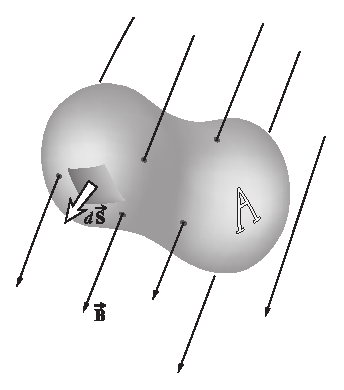
\includegraphics[width=0.5\linewidth]{Pictures/chap08/GausssLawMagnetic.eps}
    \caption{穿过封闭区域$A$的磁场$\vec{\mathbf{B}}$.}
    \label{fig:08ex02.0308}
\end{figure}

\subsubsection*{安培环路定律}


{\noindent\hfil$=========$\hfil{\color{red}{施工分割线}}\hfil$=========$\
